\exercisegroup

\begin{enumerate}
\def\labelenumi{\arabic{enumi})}
\item
  设 \(\mathrm{F}, \mathrm{G}\) 是处于对偶中的两个向量空间，且 \(\sigma(\mathrm{F}, \mathrm{G})\) 是 Hausdorff 的。证明：如果 \(\mathcal{T}\) 是一个与 \(\mathrm{F}\) 的向量空间结构相容的 Hausdorff 拓扑，并且粗于 \(\sigma(\mathrm{F}, \mathrm{G})\) （但先验地未必局部凸），那么 \(\mathcal{T} = \sigma(\mathrm{F}, \mathrm{G}_1)\) ，其中 \(\mathrm{G}_1\) 是 G 的一个向量子空间，它在拓扑 \(\sigma(\mathrm{G},\mathrm{F})\) 中稠密。（在 F 上考虑这样的局部凸拓扑 \(T_{1}\) ：其 0 的一个基本邻域系由 T 中那些闭的、凸的、均衡的且为 \(\sigma(\mathrm{F},\mathrm{G})\) 之 0 邻域的集组成。）由此推出：如果 \(T_{0}\) 是向量空间 E 上的一个 Hausdorff 局部凸拓扑，它在 E 上的 Hausdorff 局部凸拓扑所成之集中是极小的（II, 第 85 页, 习题 13），那么它在由与 E 的向量空间结构相容的 Hausdorff 拓扑（无论局部凸与否）所成之集中也是极小的。
\item
  在 \(\mathbf{R}^n\) 中，设 \((\mathrm{C}_i)_{1\leqslant i\leqslant m}\) 是由 \(m\geqslant n + 1\) 个以 0 为顶点的凸锥组成的族；证明：如果对这些锥中任何 \(n + 1\) 个锥，都存在一个过 0 的超平面 \(\mathbf{H}\) ，使这些锥位于 \(\mathbf{H}\) 的同侧，那么存在一个超平面 \(\mathrm{H}_0\) ，使所有的锥 \(\mathrm{C}_i(1\leqslant i\leqslant m)\) 都位于 \(\mathrm{H}_0\) 的同侧（参见 II, 第 68 页, 习题 21, a)）。
\item
  在 \(\mathbf{R}^n\) 中，设 \((\mathrm{D}_i)_{1\leqslant i\leqslant m}\) 是由 \(m\geqslant 2n\) 个由过 0 的超平面所确定的闭半空间组成的族。证明：如果对这些半空间中任何 \(2n\) 个，其交中存在一个 \(\neq 0\) 的点，那么存在一个 \(\neq 0\) 的点，它属于所有 \(\mathrm{D}_i(1\leqslant i\leqslant m)\) 的交（参见 II, 第 66 页, 习题 10）。
\item
  设 S、T 是 \(R^{n}\) 中两个没有公共点的有限集，且它们的并至少含 \(2n + 2\) 个点。那么，存在分离 S 与 T 的超平面，其充要条件是：对每个有限集 \(F \subset S \cup T\) （由 \(2n + 2\) 个点组成），都存在分离 \(F \cap S\) 与 \(F \cap T\) 的超平面（利用习题 3 以及 II, 第 78 页, 习题 15 的方法）。
\item
  设 E 是 \(R^{n}\) 上二次型所成的向量空间，它等同于 R 上 n 阶方阵所成空间 \(\mathbf{M}_{n}(\mathbf{R})\) 中由对称方阵组成的向量子空间。我们给 \(\mathbf{M}_{n}(\mathbf{R})\) 装备内积 \(\operatorname{Tr}(^{t}\mathbf{X},\mathbf{Y})\) ，借此可把它与其对偶等同起来；对 E 亦同样处理。
\end{enumerate}

\begin{enumerate}
\def\labelenumi{\alph{enumi})}
\item
  设 \(\mathbf{P} \subset \mathbf{E}\) 是其矩阵的元素全 \(\geqslant 0\) 的二次型所成之集，\(\mathbf{S} \subset \mathbf{E}\) 是 \(\mathbf{R}^n\) 中正二次型所成之集。证明：\(\mathbf{P} = \mathbf{P}^\circ\) ，且 \(\mathbf{S} = \mathbf{S}^\circ\) 。
\item
  设 B 是 \(\mathbf{R}^n\) 上形如 \(\sum_{j=1}^{m} x_j'^2\) （对某个 \(m\) ）的二次型所成之集，其中 \(x_{j}^{\prime}\) 是取值 \(\geqslant 0\) 的线性型——对一切向量 \(x = (x_{i})_{1\leqslant i\leqslant n}\) （其坐标 \(x_{i}\) 全 \(\geqslant 0\) ）而言；设 \(C\) 是对所有向量取值 \(\geqslant 0\) 的二次型所成之集，这里向量 \(x = (x_{i})\) 的坐标 \(x_{i}\) 全 \(\geqslant 0\) 。证明：\(B = C^{\circ}\) 且 \(C = B^{\circ}\) （证明 \(B\) 是闭的：证明 \(B\) 的每个元素都可写成形式 \(\sum_{j=1}^{m} x_{j}^{\prime 2}\) ，其中 \(x_{j}^{\prime}\) 对一切 \(x\) （坐标 \(\geqslant 0\) ）为正，且 \(m \leqslant 2^{n}\) ）。
\end{enumerate}

\begin{enumerate}
\def\labelenumi{\arabic{enumi})}
\setcounter{enumi}{5}
\tightlist
\item
  设 F、G 是处于分离对偶中的两个向量空间，A 是 F 中一个弱紧凸集。设 C 是 G 中一个以 0 为顶点且弱闭的凸锥。假设对一切 \(y \in \mathbf{C}\) ，存在 \(x \in \mathbf{A}\) 使 \(\langle x, y \rangle \geqslant 0\) 。证明：存在 \(x_0 \in \mathbf{A}\) ，使 \(\langle x_0, y \rangle \geqslant 0\) 对一切 \(y \in \mathbf{C}\) 成立（对 A 与 \(\mathbf{C}^\circ\) 应用 II, 第 38 页, prop. 4）。
\end{enumerate}

¶ 7) a) 设 F、G 是处于分离对偶中的两个向量空间，C 是 F 中一个弱闭凸锥。设 M 是 G 的一个有限维向量子空间。证明：或者存在 \(y_0 \in \mathbf{C}\) ，使 \(y_0 \in \mathbf{M}^\circ\) 且 \(y_0 \neq 0\) ，或者存在 \(z_0 \in \mathbf{M}\) ，使 \(z_0 \in \mathbf{C}^\circ\) 且 \(z_0 \neq 0\) （对 M 的维数作归纳论证）。如果 C 不含任何直线，而上述两个性质同时成立，证明 \(z_0\) 不可能是 \(\mathbf{C}^\circ\) 的代数内点。b) 设 \((a_{ij}), (b_{ij})\) 是两个具有 \(n\) 行 \(m\) 列实元素的矩阵，且 \(a_{ij} > 0\) 对每一对 \((i,j)\) 成立。证明：存在唯一的值 \(\lambda \in \mathbf{R}\) ，使得存在两个向量 \(x = (x_j) \in \mathbf{R}^m\) 、\(y = (y_i) \in \mathbf{R}^n\) ，满足关系 \(x \neq 0, y \neq 0, x_j \geqslant 0, y_i \geqslant 0\) （对一切 \(i,j\) ），并且最后满足

\[
\lambda \sum_ {j = 1} ^ {m} a _ {i j} x _ {j} \geqslant \sum_ {j = 1} ^ {m} b _ {i j} x _ {j} \quad \text { for } \quad 1 \leqslant i \leqslant n\tag{1}
\]

\[
\lambda \sum_ {i = 1} ^ {n} a _ {i j} y _ {i} \leqslant \sum_ {i = 1} ^ {n} b _ {i j} y _ {i} \quad \text { for } \quad 1 \leqslant j \leqslant m\tag{2}.
\]

（令 \(c_{ij} = \lambda a_{ij} - b_{ij}\) （对 \(1 \leqslant i \leqslant n\) ，\(1 \leqslant j \leqslant m\) ），并令 \(c_{n + i,j} = \delta_{ij}\) （Kronecker 指标，对 \(1 \leqslant i \leqslant m\) ），证明问题归结为求一个非零向量 \(x \in \mathbf{R}^m\) 与一个非零向量 \(z = (z_i) \in \mathbf{R}^{n + m}\) ，使它们满足关系

\[
\sum_ {j = 1} ^ {m} c _ {i j} x _ {j} \geqslant 0 \quad \text { for } \quad 1 \leqslant i \leqslant n + m\tag{3}
\]

\[
\sum_ {i = 1} ^ {n + m} c _ {i j} z _ {i} = 0 \quad \text { for } \quad 1 \leqslant j \leqslant m\tag{4}
\]

以及 \(z_{i} \geqslant 0\) （对 \(1 \leqslant i \leqslant n + m\) ）。注意：如果 (3) 在某个值 \(\lambda_0\) （\(\lambda\) 的一个值）处有解，那么它对 \(\lambda \geqslant \lambda_0\) 也有解；如果 (4) 对 \(\lambda_0\) 有解，那么它对 \(\lambda \leqslant \lambda_0\) 也有解。最后利用 \(a)\) 。

\begin{enumerate}
\def\labelenumi{\arabic{enumi})}
\setcounter{enumi}{7}
\tightlist
\item
  设 \(\mathbf{T}\) 是紧空间，\(\mathbf{L}\) 是 \(\mathcal{C}(\mathbf{T};\mathbf{R})\) 的一个维数为 \(r\) 的向量子空间；给 \(\mathbf{L}\) 装备由 \(\mathcal{C}(\mathbf{T};\mathbf{R})\) 的范数诱导的范数，并给其对偶 \(\mathbf{L}^*\) 装备范数 \(\| x'\| = \sup_{\| x\| \leqslant 1} \langle x, x' \rangle\) ，于是，若 \(\mathbf{B}\) 是球 \(\| x\| \leqslant 1\) （在 \(\mathbf{L}\) 中），则 \(\mathbf{B}^\circ\) 是球 \(\| x'\| \leqslant 1\) （在 \(\mathbf{L}^*\) 中）。
\end{enumerate}

\begin{enumerate}
\def\labelenumi{\alph{enumi})}
\tightlist
\item
  对每个 \(t \in \mathbf{T}\) ，用 \(e_t'\) 表示线性型 \(x \mapsto x(t)\) （\(\mathbf{L}\) 上的）。证明：\(\mathbf{B}^\circ\) 是诸 \(\pm e_t'\) 所成之集的凸包，其中 \(t\) 取遍 \(\mathbf{T}\) （利用 II, 第 38 页, prop. 4 得出矛盾）。
\end{enumerate}

由此推出：每个线性型 \(x' \in \mathbf{L}^*\) （满足 \(\| x' \| = 1\) ）都可写成 \(x' = \sum_{i=1}^{r} \lambda_i e_{t_i}'\) ，其中

诸 \(t_i\) 是 \(r\) 个属于 \(\mathbf{T}\) 的点，诸 \(\lambda_i\) 是实数，满足 \(\sum_{i=1}^{r} |\lambda_i| = 1\) （参见 II, 第 66 页, 习题 9, a)）。

\begin{enumerate}
\def\labelenumi{\alph{enumi})}
\setcounter{enumi}{1}
\tightlist
\item
  对每个 \(y \in \mathcal{C}(\mathbf{T}; \mathbf{R})\) ，存在唯一的 \(x \in \mathbf{L}\) 使 \(\| y - x \| = d(y, \mathbf{L})\) ，其充要条件是：对每个非零的 \(z \in \mathbf{L}\) ，至多存在 \(r - 1\) 个互异的点 \(t_i \in \mathbf{T}\) 使 \(z(t_i) = 0\) （Haar 定理）。（为证此条件是充分的，首先注意它等价于说：对 \(r\) 个互异的点 \(t_i \in \mathbf{T}\) （ \(1 \leqslant i \leqslant r\) ），诸 \(e_{t_i}'\) 在 \(\mathbf{L}^*\) 中线性无关。然后通过假设结论不真并得出矛盾来论证。如果存在两个互异的点 \(x', x''\) （属于 \(\mathbf{L}\) ）使 \(\| y - x' \| = \| y - x'' \| = d(y, \mathbf{L})\) ，那么存在 \(x_0 \in \mathbf{L}\) 与 \(z \in \mathbf{L}\) ，使得对一切充分小的实数 \(\lambda\) ，有 \(\| y - (x_0 + \lambda z) \| = d(y, \mathbf{L})\) 。把 \(a\) ) 的最后一部分应用于子空间 \(\mathbf{L} \oplus \mathbf{R}y\) （\(\mathcal{C}(\mathbf{T}; \mathbf{R})\) 的）以及该空间上一个在 \(\mathbf{L}\) 上为零的适当线性型。为看出该条件是必要的，注意若它不真，则存在 \(r\) 个互异的点 \(t_i \in \mathbf{T}\) （ \(1 \leqslant i \leqslant r\) ），使诸 \(e_{t_i}'\) 线性相关，且存在一个非零的函数 \(z \in \mathbf{L}\) ，它在诸点 \(t_i\) 处为零。若 \(\alpha_i (1 \leqslant i \leqslant r)\) 是不全为零的数，使 \(\sum_{i=1}^{r} \alpha_i e_{t_i}' = 0\) ，则考虑一个函数 \(w \in \mathcal{C}(\mathbf{T}; \mathbf{R})\) ，使 \(\| w \| = 1\) ，\(w(t_i) = \text{sgn}(\alpha_i)\) （对 \(1 \leqslant i \leqslant r\) ），以及函数 \(y = w(1 - |\beta z|)\) ，其中 \(|\beta|\) 充分小且 \(\neq 0\) 。）
\item
  设 \(T\) 是 \(R\) 中的一个紧区间，且 \(L\) 满足 Haar 定理的条件；设 \((t_i)_{1 \leqslant i \leqslant r+1}\) 是由 \(r + 1\) 个属于 \(T\) 的点组成的严格递增序列；则存在 \(r + 1\) 个非零实数 \(\lambda_i\) ，使 \(\sum_{i=1}^{r+1} \lambda_i e_{t_i}' = 0\) 。证明此时 \(\text{sgn}(\lambda_i) \text{sgn}(\lambda_{i+1}) = -1\) 对 \(1 \leqslant i \leqslant r\) 成立。（分别考虑 \(r = 1\) 与 \(r > 1\) 两种情形。在第二种情形，相反地假设：对某个指标 \(i \leqslant r - 1\) ，数 \(\lambda_i\) 与 \(\lambda_{i-1}\) 或与 \(\lambda_{i+1}\) 同号，且 \(\lambda_{i-1}\) 与 \(\lambda_{i+1}\) 异号。若例如 \(\lambda_i > 0\) ，取 \(\alpha_{i-1} > 0\) 、\(\alpha_{i+1} > 0\) 使 \(\alpha_{i-1} \lambda_{i-1} + \alpha_{i+1} \lambda_{i+1} = 0\) ，再取 \(z \in L\) 使 \(z(t_{i-1}) = \alpha_{i-1}\) 、\(z(t_{i+1}) = \alpha_{i+1}\) ，且 \(z(t_j) = 0\) ，其中 \(j\) 异于 \(i - 1, i\) 与 \(i + 1\) 。推出 \(z(t_i) < 0\) ，并证明这与所给假设矛盾。）
\end{enumerate}

\(d)\) ）在与 \(c\) ) 相同的假设与记号下，设存在 \(y \in \mathcal{C}(\mathrm{T}; \mathbf{R})\) 与 \(z \in \mathrm{L}\) ，使 \(y(t_i) - z(t_i) = (-1)^i \alpha_i\) ，其中 \(\alpha_i > 0\) （对 \(1 \leqslant i \leqslant r + 1\) ）。证明此时有 \(d(y, \mathrm{L}) \geqslant \inf \alpha_i\) 。（把 \(a\) ) 应用于 \(\mathrm{L} \oplus \mathbf{R}y\) ，并用 \(c\) 。）

\begin{enumerate}
\def\labelenumi{\alph{enumi})}
\setcounter{enumi}{4}
\tightlist
\item
  在 \(c\) ) 的假设下，设 \(y \in \mathcal{C}(\mathbf{T};\mathbf{R})\) ，并设 \(z\) 是 \(\mathbf{L}\) 中使 \(\| y - z \| = d(y,\mathbf{L})\) 的唯一点。证明：存在一个严格递增序列 \((t_i)_{1\leqslant i\leqslant r + 1}\) （在 \(\mathbf{T}\) 中），使得
\end{enumerate}

\[
y (t _ {i}) - z (t _ {i}) = (- 1) ^ {i} \varepsilon \| y - z \|
\]

其中 \(\varepsilon = \pm 1\) 。反之，若 \(z\) 具有此性质，则 \(z\) 是 \(\mathbf{L}\) 中使 \(\| y - z \| = d(y, \mathbf{L})\) 的唯一点。（利用 \(c\) ) 与 \(d\) ）。考察 \(\mathbf{T}\) 是 \(\mathbf{R}\) 的一个区间且 \(\mathbf{L}\) 是限制到 \(\mathbf{T}\) 上的、次数 \(< r\) 的多项式所成之集的情形（\(Tchebycheffs\) 定理）。

\begin{enumerate}
\def\labelenumi{\arabic{enumi})}
\setcounter{enumi}{8}
\tightlist
\item
  设 \(\mathbf{F}\) 与 \(\mathbf{G}\) 是处于分离对偶中的两个向量空间，\(\mathbf{A}\) 是 \(\mathbf{F}\) 的一个包含 0 的凸子集。对每个 \(y \in \mathbf{G}\) ，令
\end{enumerate}

\[
\mathrm{H} _ {\mathbf {A}} (y) = \sup _ {x \in \mathbf {A}} (- \langle x, y \rangle),
\]

于是 \(0 \leqslant \mathrm{H}_{\mathbf{A}}(y) \leqslant +\infty\) ；我们称 \(\mathrm{H}_{\mathbf{A}}\) 为 \(\mathbf{A}\) 的支撑函数。

\begin{enumerate}
\def\labelenumi{\alph{enumi})}
\item
  证明：\(\mathbf{H}_{\mathrm{A}}\) 是 \(\mathbf{A}^{\circ}\) 的度规（II, 第 20 页）。
\item
  如果 A 是弱紧的，那么对一切 \(y \in \mathbf{G}\) ，方程为 \(\langle x, y \rangle = \mathrm{H}_{\mathbf{A}}(y)\) 的超平面是 A 的一个支撑超平面。
\item
  \(\mathbf{H}_{\mathrm{A}}\) 对拓扑 \(\sigma (\mathbf{G},\mathbf{F})\) 而言有限且连续，其充要条件是 A 有限维且有界（在它所生成的有限维向量子空间中）。
\end{enumerate}

\(d\) ) 设 \(\mathbf{A}_i(1\leqslant i\leqslant p)\) 是 F 中包含 0 的凸集，\(\lambda_{i}\) 是 \(\geqslant 0(1\leqslant i\leqslant p)\) 的实数；证明凸集 \(\mathbf{A} = \sum_{i}\lambda_{i}\mathbf{A}_{i}\) 的支撑函数是 \(\mathrm{H}_{\mathrm{A}} = \sum_{i}\lambda_{i}\mathrm{H}_{\mathrm{A}_{i}}\) 。如果 \(y\in \mathbf{G}\) 使得

交集 \(C_{i}\) （即 \(A_{i}\) 与超平面 \(\langle x, y \rangle = H_{A}(y)\) 之交）对 \(1 \leqslant i \leqslant p\) 非空，证明 A 与方程为 \(\langle x, y \rangle = H_{A}(y)\) 的超平面之交就是集合 \(\sum \lambda_{i}C_{i}\) 。

\begin{enumerate}
\def\labelenumi{\alph{enumi})}
\setcounter{enumi}{4}
\item
  设 \(\mathbf{A}\) 局部紧且不含任何直线。那么，由 \(\{0\}\) 与诸 \(y \neq 0\) （它们满足 \(\mathrm{H}_{\mathrm{A}}(y) = +\infty\) ，\(\mathrm{H}_{\mathrm{A}}(-y) \neq +\infty\) ）所成之集的并，是渐近锥 \(\mathrm{C}_{\mathrm{A}}\) 的极锥（考察 \(\mathbf{A}\) 是 \(\{0\}\) 与一条半直线之凸包的情形）。
\item
  设 F 有限维。证明：A 是抛物的（II, 第 67 页, 习题 17），其充要条件是 \(H_{A}\) 是 G 到 \(\overline{R}\) 中的一个连续映射（如果存在一条平行于 \(C_{A}\) 的某条半直线且不与 A 相交的直线，注意存在一个分离该半直线与 A 的超平面）。
\end{enumerate}

\begin{enumerate}
\def\labelenumi{\arabic{enumi})}
\setcounter{enumi}{9}
\tightlist
\item
  对 \(E = R^{n}\) 中每个包含 0 的紧凸集 A，我们借助 E 与 E* 之间的对偶，使它的支撑函数 \(H_{A}\) 与之对应：\(E^{*} : H_{A}\) 属于空间 \(\mathcal{C}(E^{*}; \mathbf{R})\) ，即 \(E^{*}\) 上连续实值函数所成之空间。我们给空间 \(\mathcal{C}(E^{*}; \mathbf{R})\) 装备紧收敛的一致结构，并给 E 中包含 0 的紧凸集所成之集 \(\Re_{0}^{\prime}(E)\) 装备 II, 第 71 页, 习题 39 中定义的一致结构。证明：\(A \mapsto H_{A}\) 是 \(\Re_{0}^{\prime}(E)\) 到 \(\mathcal{C}(E^{*}; \mathbf{R})\) 的一个一致子空间上的同构。
\end{enumerate}

由此推出：映射 \(\mathbf{A} \mapsto \mathbf{A}^{\circ}\) （由集 \(\Re_0(\mathbf{E})\) ——即 \(\mathbf{E}\) 中以 0 为内点的紧凸集全体——到集 \(\Re_0(\mathbf{E}^*)\) 上）对这两个空间的一致结构而言是同构（参见 II, 第 71 页, 习题 39）。

\begin{enumerate}
\def\labelenumi{\arabic{enumi})}
\setcounter{enumi}{10}
\tightlist
\item
  设 \(\mathrm{F}, \mathrm{G}\) 是处于分离对偶中的两个向量空间。\(\mathfrak{U}\) 是 \(\mathrm{F}\) 上的一个超滤子，它弱收敛于一点 \(x_0\) 的充要条件是：\(x_0\) 属于所有属于 \(\mathfrak{U}\) 的弱闭凸集之交（注意：若 \(x_0\) 是该交中一点而非 \(\mathfrak{U}\) 的聚点，则存在一个属于 \(\mathfrak{U}\) 且不含 \(x_0\) 的闭半空间）。
\end{enumerate}

由这一结果推出：为使 F 的点列 \((x_{n})\) 弱收敛于一点 a，必要且充分的是：a 属于由该序列的无穷多项所成之集的诸弱闭凸包（利用 GT, I, § 6.4 的 prop. 7）。

\begin{enumerate}
\def\labelenumi{\arabic{enumi})}
\setcounter{enumi}{11}
\tightlist
\item
  \begin{enumerate}
  \def\labelenumii{\alph{enumii})}
  \tightlist
  \item
    设 E 是一个向量空间，\((\mathrm{E}_{\alpha})_{\alpha\in\mathrm{A}}\) 是 E 的子空间的一个递增定向族，其并为 E；设每个 \(E_{\alpha}\) 上带有一个局部凸拓扑 \(T_{\alpha}\) ，使得对 \(\alpha\leqslant\beta\) ，典范单射 \(E_{\alpha}\to E_{\beta}\) 连续。设 T 是 E 上的拓扑，它是诸 \(T_{\alpha}\) 的归纳极限（II, 第 29 页, 例 II）；证明：E 的对偶 \(E'\) （对 T 而言）带拓扑 \(\sigma(\mathrm{E}',\mathrm{E})\) 可以典范地等同于诸对偶 \(E'_{\alpha}\) 带拓扑 \(\sigma(\mathrm{E}'_{\alpha},\mathrm{E}_{\alpha})\) 的投影极限。
  \end{enumerate}
\end{enumerate}

\begin{enumerate}
\def\labelenumi{\alph{enumi})}
\setcounter{enumi}{1}
\tightlist
\item
  设 \((\mathbf{X}_{\alpha},\phi_{\alpha \beta})\) 是与指标的一个定向集 A 相对应的非空集合的投影体系，使得诸 \(\phi_{\alpha \beta}\) 都是满射且 \(\varprojlim \mathbf{X}_{\alpha} = \emptyset\) \((\mathbf{S},\mathbf{III},\S 7,\text{exerc. }4)\) 。令 \(\mathbf{F}_{\alpha} = \mathbf{R}^{(\mathbf{X}_{\alpha})}\) ，并用 \(f_{\alpha \beta}:\mathrm{F}_{\beta}\to \mathrm{F}_{\alpha}\) （对 \(\alpha \leqslant \beta\) ）表示从 \(\phi_{\alpha \beta}\) 典范地导出的线性映射（A, II, § 1.11, cor. 1）。如果我们给每个 \(\mathbf{F}_{\alpha}\) 装备其因子的直和拓扑，那么对偶 \(\mathrm{E}_{\alpha} = \mathrm{F}_{\alpha}'\) （\(\mathrm{F}_{\alpha}\) 的对偶）带弱拓扑 \(\sigma(\mathrm{E}_{\alpha}, \mathrm{F}_{\alpha})\) 可以等同于乘积空间 \(\mathbf{R}^{\mathbf{X}_{\alpha}}\) ，且 \({}^{t}f_{\alpha\beta}\) 是 \(\mathrm{E}_{\alpha}\) 到 \(\mathrm{E}_{\beta}\) 的一个闭子空间上的同构，该子空间在 \(\mathrm{E}_{\beta}\) 中有拓扑补。证明：在 \(\mathrm{E} = \varinjlim \mathrm{E}_{\alpha}\) 上（对诸 \({}^{t}f_{\alpha\beta}\) 而言），诸 \(\mathrm{E}_{\alpha}\) 的拓扑的归纳极限是最粗的拓扑（从而非 Hausdorff）（利用 \(a\) 并注意到 \(\varprojlim \mathrm{F}_{\alpha} = \{0\}\) ）。
\end{enumerate}

\begin{enumerate}
\def\labelenumi{\arabic{enumi})}
\setcounter{enumi}{12}
\tightlist
\item
  设 E 是一个向量空间。我们称 E 上的一个 Hausdorff 局部凸拓扑 T 是极小的（并称带 T 的 E 是极小型空间），如果在 E 上不存在严格粗于 T 的 Hausdorff 局部凸拓扑（参见 II, 第 81 页, 习题 1）。
\end{enumerate}

\begin{enumerate}
\def\labelenumi{\alph{enumi})}
\item
  设 \(\mathcal{T}\) 是 E 上的一个极小拓扑，并设 \(E'\) 是 E 的对偶（当 E 带拓扑 \(\mathcal{T}\) 时）；证明 \(\mathcal{T} = \sigma(E, E')\) 且 \(E = E'^*\) （注意：利用 II, 第 43 页的推论 3，在 \(E'\) 中对拓扑 \(\sigma(E', E)\) 不可能存在处处稠密的超平面）。由此推出极小型空间是直线的乘积。
\item
  证明：在 Hausdorff 局部凸空间 F 中，每个极小型的子空间 E 都有拓扑补，从而特别地是闭的（利用 a) 以及 Hahn--Banach 定理，把 E 到自身的恒等映射延拓为 F 到 E 的一个映射）。
\item
  设 \(u\) 是从极小型空间 \(\mathbf{E}\) 到 Hausdorff 局部凸空间 \(\mathbf{F}\) 的一个连续线性映射。证明：\(u(\mathbf{E})\) 在 \(\mathbf{F}\) 中闭，且 \(u\) 是 \(\mathbf{E}\) 到 \(\mathbf{F}\) 的严格态射（利用 \(b\) 以及极小型空间的定义）。
\item
  设 F 是 Hausdorff 局部凸空间，M 是 F 的一个闭向量子空间。证明：如果存在 M 在 F 中的一个补 N，它是极小型的子空间，那么 N 是 M 在 F 中的拓扑补（利用 c)）。
\item
  设 M 是 Hausdorff 局部凸空间 F 中的一个极小型子空间；证明：对 F 的每个闭向量子空间 N，和 \(M + N\) 在 F 中闭（考察商空间 F/N 并利用 c)）。如果进而 N 也是极小型的，那么 \(M + N\) 是极小型的。
\end{enumerate}

\begin{enumerate}
\def\labelenumi{\arabic{enumi})}
\setcounter{enumi}{13}
\tightlist
\item
  设 \(\mathbf{E}\) 是 Hausdorff 局部凸空间，\(\mathbf{F}\) 是极小型的局部凸空间（习题 13）。
\end{enumerate}

\begin{enumerate}
\def\labelenumi{\alph{enumi})}
\item
  证明：如果 \(\mathbf{M}\) 是乘积空间 \(\mathrm{E} \times \mathrm{F}\) 的一个闭向量子空间，则它在 \(\mathrm{E}\) 上的投影在 \(\mathrm{E}\) 中闭（利用习题 13, e)）。
\item
  设 \(u\) 是 \(\mathbf{E}\) 到 \(\mathbf{F}\) 的一个线性映射。证明：如果 \(u\) 的图像在 \(\mathbf{E} \times \mathbf{F}\) 中闭，那么 \(u\) 连续（利用 \(a\) ）。
\item
  假设在 E 中每个闭向量子空间都有拓扑补（参见 V, 第 13 页）。证明：在 \(E \times F\) 中，每个闭向量子空间 M 都有拓扑补。（如果 \(N_{1}\) 是 M 在 E 上的投影，\(N_{2}\) 是 \(N_{1}\) 在 E 中的一个拓扑补，如果 \(P_{1} = M \cap F\) ，而 \(P_{2}\) 是 \(P_{1}\) 在 F 中的一个拓扑补，试利用 b) 证明 \(N_{2} + P_{2}\) 是 M 在 \(E \times F\) 中的一个拓扑补。）
\end{enumerate}

* 15) 设 E, F 是两个 Hausdorff 局部凸空间。我们称连续线性映射 \(u: \mathrm{E} \to \mathrm{F}\) 是线性真的，如果对每个 Hausdorff 局部凸空间 G 和 \(\mathrm{E} \times \mathrm{G}\) 的每个闭向量子空间 V，V 在映射 \(u \times 1_{\mathrm{G}}: \mathrm{E} \times \mathrm{G} \to \mathrm{F} \times \mathrm{G}\) 下的像是闭的。证明：这一条件等价于下述条件：\(u^{-1}(0)\) 是 E 的一个极小型子空间，且对 E 的每个闭向量子空间 W，集合 \(u(\mathbf{W})\) 在 F 中闭。（为证明第一个条件蕴含第二个，考察映射 \(v: \mathrm{E} \to \{0\}\) ，并给 E 装备拓扑 \(\sigma(\mathrm{E}, \mathrm{E}')\) ，使 E 浸入 \(\mathrm{E}'*\) 中且带拓扑 \(\sigma(\mathrm{E}'*, \mathrm{E}')\) ，然后取投影 \(v \times 1_{\mathrm{E}'*}: \mathrm{E} \times \mathrm{E}'* \to \mathrm{E}'*\) 下的像，这里所取的是 \(\mathrm{E} \times \mathrm{E}'*\) 中对角线 \(\Delta\) （\(\mathrm{E} \times \mathrm{E}\) 的对角线）的闭包。为证明第二个条件蕴含第一个，证明它蕴含：对拓扑 \(\sigma(\mathrm{E}, \mathrm{E}')\) 与 \(\sigma(\mathrm{F}, \mathrm{F}')\) 而言，映射 \(u\) 是严格态射，并利用习题 13, e)。) *

\begin{enumerate}
\def\labelenumi{\arabic{enumi})}
\setcounter{enumi}{15}
\tightlist
\item
  设 \(\mathbf{F}\) 是直线的乘积，\(\mathbf{C}\) 是 \(\mathbf{F}\) 中的一个闭凸集。
\end{enumerate}

\begin{enumerate}
\def\labelenumi{\alph{enumi})}
\item
  证明：存在 \(x_0 \in \mathbf{F}\) 、两个集合 I 与 J，以及一个拓扑同构 \(u\) （从 \(\mathbf{F}\) 到 \(\mathbf{R}^{\mathbf{I}} \times \mathbf{R}^{\mathbf{J}}\) 上的），使得 \(u(x_0 + \mathbf{C})\) 形如 \(\mathbf{R}^{\mathbf{I}} \times \mathbf{A}\) ，其中 \(\mathbf{A}\) 是 \(\mathbf{R}_+^{\mathbf{J}}\) 中的一个闭凸集。（注意我们有 \(\mathbf{F} = \mathbf{G}^*\) ，这里 \(\mathbf{F}\) 带拓扑 \(\sigma(\mathbf{G}^*, \mathbf{G})\) ；考察极集 \(C^\circ\) （\(C\) 在 \(G\) 中的极集）、\(G\) 中由 \(C^\circ\) 生成的向量子空间，以及该子空间的一个补。）
\item
  如果 C 不含任何仿射直线，那么 \((x, y) \mapsto x + y\) （从 \(C \times C\) 到 \(F\) 的映射）是真映射。
\item
  假设 C 是以 0 为顶点的锥，且由 F 的一致结构在 C 上诱导的一致结构是可度量化的。那么，如果集合 I 与 J、点 \(x_0\) 和映射 \(u\) 满足 \(a\) ) 的条件，则 I 是可数的，且存在 J 的一个可数子集 H，使得典范投影 \(p: \mathbf{R}^{\mathrm{I}} \times \mathbf{R}^{\mathrm{J}} \to \mathbf{R}^{\mathrm{I}} \times \mathbf{R}^{\mathrm{H}}\) 到 \(u(x_0 + \mathbf{C})\) 上的限制是一致子空间 \(u(x_0 + \mathbf{C})\) （\(\mathbf{R}^{\mathrm{I}} \times \mathbf{R}^{\mathrm{J}}\) 中的一致子空间）到一致子空间 \(p(u(x_0 + \mathbf{C}))\) （\(\mathbf{R}^{\mathrm{I}} \times \mathbf{R}^{\mathrm{H}}\) 中的一致子空间）上的同构。
\end{enumerate}

\begin{enumerate}
\def\labelenumi{\arabic{enumi})}
\setcounter{enumi}{16}
\tightlist
\item
  设 \(\mathbf{E}\) 是一个无限维向量空间。
\end{enumerate}

\begin{enumerate}
\def\labelenumi{\alph{enumi})}
\tightlist
\item
  证明：在 \(\mathrm{E}^*\) 中存在对拓扑 \(\sigma (\mathrm{E}^{*},\mathrm{E})\) 处处稠密的超平面。b) 如果 \(\mathbf{H}'\) 是这样一个超平面，证明：在 E 中，\(\neq \mathrm{E}\) 的、对拓扑 \(\sigma (\mathrm{E},\mathrm{H}')\) 处处稠密的线性子流形只有超平面。
\end{enumerate}

  ¶ 18) a) 在赋范空间 E 中，设 A 是一个闭凸集且 \(\neq\) E；证明函数 \(x\mapsto d(x,\complement\mathbf{A})\) 在 A 中是凹的（利用 A 是诸闭半空间之交这一事实）。b) 按下述方式归纳地定义闭凸集的一个序列 \(\mathbf{A}_{n}\subset\mathbf{R}^{n}\) ：\(\mathbf{A}_{1}=\mathbf{R}_{+}\) ；如果把 \(\mathbf{R}^{n+1}\) 等同于 \(\mathbf{R}^{n}\times\mathbf{R}\) ，那么 \(\mathbf{A}_{n+1}\) 是这样的偶 \((x,\xi)\) 所成之集：\(x\in\overset{\circ}{\mathbf{A}}_{n}\) 以及

\[
\xi \geqslant (d (x, \complement A _ {n})) ^ {- 1} + \| x \| ^ {2},
\]

其中 \(\|x\|\) 是欧氏范数。证明：\(A_{n+1}\) 没有任何形如 \(H \times R\) 的支撑超平面（这里 H 是 \(R^{n}\) 的一个超平面），且它的渐近锥是 \(\{0\} \times R_{+}\) 。c) 如果 \(p_{nm}\) 是典范投影 \(R^{m} \to R^{n}\) （把 \(R^{m}\) 等同于 \(R^{n} \times R^{m-n}\) ，对 \(m \geqslant n\) ），证明：当 \(R^{N}\) 等同于投影体系 ( \(R^{n}, p_{nm}\) ) 的投影极限时，诸 \(A_{n}\) 构成集合的一个投影体系，且 \(A = \varprojlim A_{n}\) 是 \(R^{N}\) 中一个非相对紧的闭凸集，它没有闭的支撑超平面，并且 \(C_{A} = \{0\}\) 。

\begin{enumerate}
\def\labelenumi{\arabic{enumi})}
\setcounter{enumi}{18}
\tightlist
\item
  \begin{enumerate}
  \def\labelenumii{\alph{enumii})}
  \tightlist
  \item
    设 A 是 E（直线的乘积）中一个非紧的闭凸集，且 \(C_{A} = \{0\}\) （习题 18）。证明：如果 \(B = \overline{A - A}\) ，且 M 是 \(A \cup (-A)\) 的闭凸包，那么 B 与 M 都含直线（利用 II, 第 85 页, 习题 16, b)）。
  \end{enumerate}
\end{enumerate}

\begin{enumerate}
\def\labelenumi{\alph{enumi})}
\setcounter{enumi}{1}
\tightlist
\item
  设 \(\mathrm{A}_1, \mathrm{A}_2\) 是 E 中两个闭凸集，使得 \(\mathrm{A}_1 + \mathrm{A}_2\) 闭，且 \(\mathrm{A}_1\) 、\(\mathrm{A}_2, \mathrm{A}_1 + \mathrm{A}_2\) 中没有一个含仿射直线。证明 \(\mathrm{C}_{\mathrm{A}_1 + \mathrm{A}_2} = \mathrm{C}_{\mathrm{A}_1} + \mathrm{C}_{\mathrm{A}_2}\) （利用 II, 第 85 页, 习题 16, b)）。c) 设 A 是 E 中不含任何仿射直线的一个闭凸集，而 \(\mathbf{M}_1, \dots, \mathbf{M}_n\) 是含于 A 中的闭凸集。如果 B 是 \(\bigcup_{i} \mathbf{M}_i\) 的凸包，证明 \(\overline{\mathbf{B}} = \mathbf{B} + \sum_{i} \mathbf{C}_{\mathbf{M}_i}\)
\end{enumerate}

以及 \(C_B = \sum_i C_{M_i}\) （同样的方法）。

¶ 20) 设 \(\mathrm{F} = \mathbf{R}^{(\mathrm{A})}, \mathrm{G} = \mathbf{R}^{\mathrm{A}}\) ，其中 \(\mathrm{A}\) 是任意无限集；假设 \(\mathrm{F}\) 与 \(\mathrm{G}\) 通过双线性型 \(\langle x, y \rangle = \sum_{\alpha \in \mathbf{A}} x(\alpha) y(\alpha)\) 处于分离对偶中。

\begin{enumerate}
\def\labelenumi{\alph{enumi})}
\item
  设 N 是 G 的一个加法子群；我们用 \(N^{*}\) 表示这样的 \(x \in F\) 所成的子群：\(\langle x, y \rangle\) 对所有 \(y \in N\) 都是整数；并用 \(N^{**}\) 表示这样的 \(z \in G\) 所成的子群：\(\langle x, z \rangle\) 对所有 \(x \in N^{*}\) 都是整数。如果 \(\overline{N}\) 是 N 对拓扑 \(\sigma(G, F)\) 的闭包，证明：\(N^{*}\) 在 F 中对 \(\sigma(F, G)\) 闭，且 \(N^{**} = \overline{N}\) （为确立最后一点，利用 GT, VII, § 1.3, 命题 6，把 N 投影到 G 的有限维坐标流形上）。
\item
  假设 \(\mathbf{A} = \mathbf{N}\) 。设 \(\mathbf{M}\) 是 \(\mathbf{F}\) 的一个对 \(\sigma(\mathbf{F},\mathbf{G})\) 闭的子群；证明：如果 \(\mathbf{V}\) 是含于 \(\mathbf{M}\) 中的最大向量子空间，那么 \(\mathbf{M}\) 是 \(\mathbf{V}\) 与一个闭子群 \(\mathbf{P}\) （它是一个具有可数基的自由 \(\mathbf{Z}\) -模）的拓扑直和。（把 \(\mathbf{F}\) 看作有限维向量子空间的递增序列 \((\mathrm{F}_n)\) 之并，并应用 GT, VII, § 1.2, 定理 2 与 § 1, 习题 7。）\(\mathbf{P}\) 是离散的（对由 \(\sigma(\mathbf{F},\mathbf{G})\) 诱导的拓扑而言），当且仅当 \(\mathbf{P}\) 是有限秩的。
\item
  由 a) 与 b) 推出：当 A = N 时，G 的每个闭子群（当 G 带乘积拓扑 \(\sigma(\mathbf{G}, \mathbf{F})\) 时）都可被拓扑群 G 的一个自同构变换为乘积 \(R^{I} \times Z^{J}\) ，其中 I 与 J 是 N 的两个无公共元素的集合。d) 在空间 \(E = R^{N}\) （带拓扑 \(\sigma(E, E^{*})\) ）中，证明子群 \(Z^{N}\) 是闭的且不含任何直线，尽管它不是自由 Z-模（A, VII, 第 59 页, 习题 8）；因此当 A 不可数时 b) 的结果不能推广。
\end{enumerate}

\exercisegroup

\begin{enumerate}
\def\labelenumi{\arabic{enumi})}
\item
  设 A 是一个凸集。那么，一点 \(x \in A\) 是 A 的极点，当且仅当对 A 的任何子集 B，由 x 属于 B 的凸包这一论断可推出 \(x \in B\) 。
\item
  沿用 II, 第 74 页, 习题 3 的记号，设 G 是 E 中由 K ∪ \{λ\} 生成的向量子空间。证明：在 G 中，点 λ 是 K 的闭凸包的一个极点，但 λ 不属于 K（参见 II, 第 25 页, 推论）。
\end{enumerate}

¶ 3) 设 A 是向量空间 E 中的一个凸集，x 是 A 的一点。我们把由 x 以及 A 中这样的 \(y \neq x\) （过 x 与 y 的直线包含一个开线段，它含于 A 且含 x）所构成的集合称为 x 在 A 中的刻面。A 的（关于由 A 生成的线性流形的）代数内点（相应地，极点）（II, 第 26 页）是指在 A 中的刻面等于 A（相应地，缩为一点）的那些点。

\begin{enumerate}
\def\labelenumi{\alph{enumi})}
\item
  证明：刻面 \(\mathrm{F}_x\) （一点 \(x \in \mathbf{A}\) 的刻面）是最大的凸集 \(\mathbf{B} \subset \mathbf{A}\) ，使得 \(x\) 是 \(\mathbf{B}\) （关于由 \(\mathbf{B}\) 生成的线性流形）的代数内点。
\item
  对每一点 \(y \in \mathbf{F}_x\) ，刻面 \(\mathbf{F}_y\) （\(y\) 在 \(\mathbf{A}\) 中的刻面）与 \(y\) 在 \(\mathbf{F}_x\) 中的刻面恒同。要使 \(\mathbf{F}_y = \mathbf{F}_x\) ，必须且只需 \(y\) 是 \(\mathbf{F}_x\) （关于由 \(\mathbf{F}_x\) 生成的线性流形）的代数内点。由此推出：如果 \(\mathbf{F}_x\) 是有限维的，且 \(y\) 是 \(\mathbf{F}_x\) （关于由 \(\mathbf{F}_x\) 生成的线性流形）的非代数内点，那么 \(\mathbf{F}_y\) 的维数严格小于 \(\mathbf{F}_x\) 的维数。
\item
  E 中与 A 相交且满足下述条件的线性流形 V 称为 A 的支撑流形：对每个 \(x \in A \cap V\) ，每个含于 A 且含 x 的开线段必然含于 V。证明：对所有 \(x \in A\) ，由 x 在 A 中的刻面 \(F_{x}\) 生成的线性流形 M 是包含 x 的最小支撑流形，且 \(M \cap A = F_{x}\) 。对 A 的每个支撑流形 V，交 \(V \cap A\) 是它的每个代数内点（关于由 \(V \cap A\) 生成的线性流形）在 A 中的刻面。
\end{enumerate}

\(d\) ) 设 \(\mathbf{A}\) 与 \(\mathbf{B}\) 是 \(\mathbf{E}\) 中两个凸集。对每一点 \(x\in \mathbf{A}\cap \mathbf{B}\) ，\(x\) 在 \(\mathbf{A}\cap \mathbf{B}\) 中的刻面是 \(x\) 在 \(\mathbf{A}\) 中与在 \(\mathbf{B}\) 中诸刻面之交。

\begin{enumerate}
\def\labelenumi{\alph{enumi})}
\setcounter{enumi}{4}
\item
  设 B 是 Hausdorff 拓扑向量空间 E 中的一个闭凸集，且 B 含有一个具有有限余维数 n 的闭线性流形 M；那么 B 的每一点在 B 中的刻面都含有一个余维数为 n 的闭线性流形（II, 第 67 页, 习题 14, d)）。如果 A 是一个凸集，那么 A ∩ B 的一点 x 在 A ∩ B 中的刻面是有限维的，当且仅当 x 在 A 中的刻面是有限维的：进而，若 p 与 q 分别是 x 在 A 中的刻面与 x 在 A ∩ B 中的刻面的维数，则 \(p \leqslant q + n\) 。特别地，如果 \(x \in A \cap B\) 是 A ∩ B 的一个极点，那么它在 A 中的刻面的维数 \(\leqslant n\) 。
\item
  由 e) 推出：如果 A 是紧的，且 V 是 E 中一个具有有限余维数 n 的闭线性流形，那么 \(V \cap A\) 的每个极点至多是 A 的 \(n + 1\) 个极点的线性组合。
\end{enumerate}

\begin{enumerate}
\def\labelenumi{\arabic{enumi})}
\setcounter{enumi}{3}
\item
  在平面 \(\mathbf{R}^2\) 中，考虑凸集 \(\mathbf{A}\) ，它由这样的点 \((\xi, \eta)\) 构成：\(-1 \leqslant \xi \leqslant 1\) ，\(-1 - \sqrt{1 - \xi^2} \leqslant \eta \leqslant 1 + \sqrt{1 - \xi^2}\) 。证明：存在 \(\mathbf{A}\) 的一些边界点，它们的刻面异于 \(\mathbf{A}\) 与过该点的 \(\mathbf{A}\) 的支撑直线之交。
\item
  在实数的有界序列所成的 Banach 空间 \(l^{\infty}(\mathbf{N})\) （其中的序列写作 \(x = (\xi_n)\) ）中，设 \(\mathbf{A}\) 是由不等式 \(-1 / n \leqslant \xi_n \leqslant 1\) （对 \(n \geqslant 1\) ）与 \(-1 \leqslant \xi_0 \leqslant 1\) 所定义的闭凸集。证明：\(\mathbf{A}\) 有非空内部，原点是 \(\mathbf{A}\) 的一个边界点，且 0 在 \(\mathbf{A}\) 中的刻面不是闭的。如果我们给 \(\mathbf{A}\) 装备由乘积空间 \(\mathbf{R}^{\mathbf{N}}\) 的拓扑诱导的拓扑，证明 \(\mathbf{A}\) 是紧的，但 0 在 \(\mathbf{A}\) 中的刻面在 \(\mathbf{A}\) 中不闭。
\item
  设 E 与 \(E'\) 是处于分离对偶中的两个向量空间，A 是 E 中包含 0 且对 \(\sigma(\mathrm{E}, \mathrm{E}')\) 闭的一个凸集。对所有 \(a \in A\) ，记 \(F_{a}'\) 为点 \(x' \in A^{\circ}\) （满足 \(\langle a, x' \rangle = -1\) ）所成之集；它是一个闭的（对 \(\sigma(\mathrm{E}', \mathrm{E})\) ）凸集，含于 \(A^{\circ}\) 。证明：\(F_{a}'\) 是 \(A^{\circ}\) 中的刻面，即 \(F_{a}'\) （关于由 \(F_{a}'\) 生成的线性流形）的每个代数内点的刻面。我们称 \(F_{a}'\) 为 a 在 \(A^{\circ}\) 中的对偶刻面。如果 \(F_{a}\) 是 a 在 A 中的刻面，证明：\(F_{a}'\) 也是在 \(A^{\circ}\) 中的对偶刻面——对 \(F_{a}\) （关于由 \(F_{a}\) 生成的线性流形）的每个代数内点而言；进而，如果把 A 等同于 \(A^{\circ\circ}\) ，那么 \(F_{a}^{\prime}\) （关于由 \(F_{a}^{\prime}\) 生成的线性流形）的每个代数内点在 A 中的对偶刻面包含 \(F_{a}\) 。当 \(F_{a}^{\prime}\) 非空时（当 E 有限维且 \(a \neq 0\) 时这总是成立的，参见 II, 第 78 页, 习题 13），我们称 \(F_{a}\) 与 \(F_{a}^{\prime}\) 中的每一个是另一个的对偶刻面。
\end{enumerate}

我们称点 \(a \in \mathbf{A}\) 是 \(\mathbf{A}\) 的光滑点，如果 \(\mathbf{F}_a'\) 缩为一点（换句话说，如果存在 \(\mathbf{A}\) 的一个过 \(a\) 的闭支撑超平面）；我们称 \(a\) 是严格凸点（或暴露点），如果存在一个闭支撑超平面 \(\mathbf{H}\) （它支撑 \(\mathbf{A}\) ），使得 \(\mathbf{H} \cap \mathbf{A} = \{a\}\) ；这等价于说：\(\mathbf{F}_a'\) （关于由 \(\mathbf{F}_a'\) 生成的某个线性流形）的一个代数内点是 \(\mathbf{A}^\circ\) 的光滑点。

\begin{enumerate}
\def\labelenumi{\arabic{enumi})}
\setcounter{enumi}{6}
\tightlist
\item
  设 \(\mathbf{E}\) 是有限维（维数 \(n\) ）的向量空间，\(\mathbf{A}\) 是 \(\mathbf{E}\) 中的一个闭凸集，0 是它的一个内点。
\end{enumerate}

\begin{enumerate}
\def\labelenumi{\alph{enumi})}
\item
  设 F 与 \(F'\) 是 A 与 \(A^{\circ}\) 的两个对偶刻面（习题 6）；如果 F 是 p 维的而 \(F'\) 是 q 维的，试证明 \(p + q \leqslant n - 1\) 。对 A 的每个边界点 x，x 在 A 中的刻面的维数称为 x 的阶，其对偶刻面在 \(A^{\circ}\) 中的维数称为 x 的类。A 的刻面 F 的阶（相应地，类）按定义是 F 的某个代数内点（关于由 F 生成的线性流形）的阶（相应地，类）。A 的极点是 0 阶点；A 的光滑点（习题 6）是 0 类点。
\item
  A 的一个 n - 1 类（从而 0 阶）的边界点称为 A 的顶点。证明：A 的顶点所成之集是可数的（考察 A 的诸顶点的对偶刻面所成之集，GT, VI, § 2, 习题 12）。
\item
  设 F 是 A 的一个 p 维刻面，M 是 n - p 维的一个线性流形，它与 F 仅交于一点 a，a 是 F 的一个代数内点，且 M 含有 A 的一个内点。证明：如果 V 是 \(M \cap A\) 在 M 中的一个过 a 的支撑超平面，那么由 \(F \cup V\) （在 E 中）生成的超平面 H 是 A 的一个支撑超平面。
\item
  我们称 A 的一个 p 阶 q 类的刻面 F 为超刻面，如果 \(p + q = n - 1\) ；此时其对偶刻面也是 \(A^{\circ}\) 的一个超刻面。如果一个 n - p 维的线性流形 M 与一个超刻面 F 仅交于一点，且该点是 F 的一个代数内点（关于由 F 生成的线性流形），证明：该点是凸集 \(M \cap A\) 的一个顶点，反之亦然（利用 c)）。由此推出：A 的 p 阶超刻面所成之集是可数的。（把 E 等同于 \(R^{n}\) ，考察 A 在 \(R^{n}\) 的每个 p 维坐标流形上的投影；如果其在一个坐标流形 V 上的投影为 p 维的那种 p 阶超刻面所成之集不可数，则借助 V 中具有有理坐标的点，证明存在 V 的一点，它是不可数无穷多个这种投影的内点；然后利用 b)。）试给出一个凸集的例子，它有不可数无穷多个刻面，其中每一个既不是单独一点也不是超刻面。
\item
  如果 A 的所有边界点都是光滑的，证明：把 A 的边界 G 的每一点 x 对应到 x 的对偶刻面的唯一点的映射，是 G 到 A° 的边界上的一个连续映射（参见 TG, I, § 9.1, 推论）。在什么情形下这个映射是双射？
\end{enumerate}

\begin{enumerate}
\def\labelenumi{\arabic{enumi})}
\setcounter{enumi}{7}
\tightlist
\item
  设 \(\mathbf{E}\) 是有限维（维数 \(n\) ）的向量空间，\(\mathbf{A}\) 是 \(\mathbf{E}\) 中的一个紧凸集。
\end{enumerate}

\begin{enumerate}
\def\labelenumi{\alph{enumi})}
\item
  设 H 是 E 中一个超平面。证明：在由 H 确定的、且至少含 A 的一点的开半空间中，存在 A 的一个严格凸点（II, 第 87 页, 习题 6）。（在 H 中考虑一个 n - 1 维的、半径充分大且包含 H ∩ A 的闭欧氏球 C，然后考虑包含 A 且满足 B ∩ H = C 的、半径更大的 n 维欧氏球 B。）
\item
  证明：A 是严格凸点所成之集的闭凸包（利用 a)）。c) 证明：A 的每个极点都是 A 的严格凸点所成之集的一个聚点。（利用 b) 与 II, 第 66 页, 习题 9, a)，注意一个极点是形如 \(\sum_{i=0}^{n} \lambda_{im} x_{im}\) 的点组成的序列的极限，其中 \(\lambda_{im} \geqslant 0\) ，\(\sum_{i=0}^{n} \lambda_{im} = 1\) ，且诸 \(x_{im}\) 是 A 的严格凸点；然后利用 A 的紧性。）
\end{enumerate}

\begin{enumerate}
\def\labelenumi{\arabic{enumi})}
\setcounter{enumi}{8}
\item
  证明：在乘积空间 \(\mathbf{E} = \mathbf{R}^{\mathbf{N}}\) 中，方体 \(\mathbf{I}^{\mathbf{N}}\) （其中 \(\mathbf{I} = [0,1]\) ）是没有严格凸点的紧凸集。
\item
  在空间 \(\mathbf{R}^2\) 中，证明：闭凸集 \(\mathbf{A}\) 的极点所成之集是闭的（证明 A 中其在 A 中的刻面为 1 维的那种点所成之集，相对于 A 的边界是开集）。
\item
  \begin{enumerate}
  \def\labelenumii{\alph{enumii})}
  \tightlist
  \item
    在空间 \(\mathbf{R}^3\) 中，考虑紧凸集 A，它是圆 \(\zeta = 0\) ，\(\xi^2 + \eta^2 - 2\xi = 0\) 与两点 \((0, 0, 1)\) 、\((0, 0, -1)\) 之并的凸包。证明：A 的极点所成之集在 A 中不闭。
  \end{enumerate}
\end{enumerate}

\begin{enumerate}
\def\labelenumi{\alph{enumi})}
\setcounter{enumi}{1}
\tightlist
\item
  设 A 是 Hausdorff 拓扑向量空间 E 中一个可度量化的紧凸集。证明：A 的极点所成之集是 A 中一列开集之交。（如果 d 是定义 A 的拓扑的一个距离，那么对每个整数 n，考虑点 \(x = \frac{1}{2}(y + z)\) 所成之集，其中 y, z 属于 A 且 \(d(y, z) \geqslant 1/n\) 。）
\end{enumerate}

\begin{enumerate}
\def\labelenumi{\arabic{enumi})}
\setcounter{enumi}{11}
\tightlist
\item
  在 Banach 空间 \(l^{\infty}(\mathbf{N})\) 中，设 \(e_n\) 是除第 \(n\) 项为 1 外其余各项均为零的序列。设 \(\mathbf{A}\) 是由 0 与诸点 \(\mathbf{e}_n / (n + 1)\) ( \(n \geqslant 0\) )所成之集的闭凸包。证明：\(\mathbf{A}\) 是紧的，但它不等同于其极点所成之集的凸包。
\end{enumerate}

* 13) 在 Hilbert 空间 \(l^2(\mathbf{N})\) 中，设 \(\mathbf{A}\) 是这样的点 \(x = (\xi_n)\) 所成之集：\(\sum_{n} 2^{2n}\xi_n^2 \leqslant 1\) 。证明：\(\mathbf{A}\) 是凸的、紧的，且它是其极点所成之集的闭包。

\begin{enumerate}
\def\labelenumi{\arabic{enumi})}
\setcounter{enumi}{13}
\tightlist
\item
  设 \(\mathbf{E}\) 是 Banach 空间 \(l^{\infty}(\mathbf{N})\) 的一个闭向量子空间，它由序列 \(x = (\xi_n)\) （满足 \(\lim_{n\to \infty}\xi_n = 0\) ）组成。
\end{enumerate}

\begin{enumerate}
\def\labelenumi{\alph{enumi})}
\tightlist
\item
  证明：在 Banach 空间 E 中，闭单位球 B 没有任何极点。b) 设 \(u\) 是 E 上的连续线性型 \((\xi_n) \mapsto \sum_n 2^{-n}\xi_n\) 。证明：不存在 B 的支撑超平面平行于方程为 \(u(x)=0\) 的闭超平面。
\end{enumerate}

\begin{enumerate}
\def\labelenumi{\arabic{enumi})}
\setcounter{enumi}{14}
\tightlist
\item
  设 \(\mathbf{A}\) 是赋范空间 \(\mathbf{E}\) 中的一个紧集。
\end{enumerate}

\begin{enumerate}
\def\labelenumi{\alph{enumi})}
\item
  证明：A 的两个平行支撑超平面之间的距离至多等于 A 的直径 \(\delta\) 。
\item
  证明：存在 A 的点偶 \((a, b)\) 使 \(\|a - b\| = \delta\) ；对这样的点偶，存在 A 的两个平行支撑超平面，分别过 a 与 b，且它们之间的距离为 \(\delta\) （考察中心在 a、半径为 \(\delta\) 的闭球）。
\end{enumerate}

\begin{enumerate}
\def\labelenumi{\arabic{enumi})}
\setcounter{enumi}{15}
\tightlist
\item
  \begin{enumerate}
  \def\labelenumii{\alph{enumii})}
  \tightlist
  \item
    设 A 是空间 \(R^{n}\) （带欧氏范数）中一个 n 维紧凸集；对每个 \(z \in S_{n-1}\) ，用 \(\rho(z)\) 表示平行于向量 z 且含于 A 的线段长度的上确界。证明：存在 A 的两点 u, v，使得端点为 u, v 的线段平行于 z 且长度为 \(\rho(z)\) ；由此推出：存在 A 的两个平行的支撑超平面，分别过 u 与 v（考察集合 \(A' = A + \rho(z)z\) ，并用一个超平面分离集合 A 与 \(A'\) ）。
  \end{enumerate}
\end{enumerate}

\begin{enumerate}
\def\labelenumi{\alph{enumi})}
\setcounter{enumi}{1}
\tightlist
\item
  设 d 是 A 的两个平行支撑超平面之间距离的下确界；证明：存在 A 的两点 a, b 使 \(\|a - b\| = d\) ，且分别过 a 与 b 并垂直于 a - b 的超平面都是 A 的支撑超平面（利用 a)）。
\end{enumerate}

\begin{enumerate}
\def\labelenumi{\arabic{enumi})}
\setcounter{enumi}{16}
\item
  在空间 \(l^{\infty}(\mathbf{N})\) 中，设 \(\mathbf{A}\) 是 II, 第 89 页, 习题 12 中定义的紧凸集，并设 \(\mathbf{E}\) 是 \(l^{\infty}(\mathbf{N})\) 中由 \(\mathbf{A}\) 生成的闭向量子空间。证明：\(\mathbf{A}\) 在空间 \(\mathbf{E}\) 中的两个平行闭支撑超平面之间距离的下确界等于 0，尽管 \(\mathbf{A}\) 并不含于 \(\mathbf{E}\) 的任何闭超平面中。
\item
  在 Hausdorff 局部凸空间 E 中，设 \((\mathbf{K}_{\alpha})_{\alpha\in\mathbf{I}}\) 是由非空紧凸集组成的一个递减定向族。对所有 \(\alpha\in I\) ，把 \(K_{\alpha}\) 的极点所成之集记作 \(A_{\alpha}\) ，并把 \(F_{\alpha}\) 记作诸 \(A_{\beta}\) （\(\beta\geqslant\alpha\) ）之并的闭包，于是 \((\mathrm{F}_{\alpha})\) 是紧集的一个递减定向族。设 A 是诸 \(F_{\alpha}\) 的（非空）交，K 是诸 \(K_{\alpha}\) 的（非空）交。证明：K 是 A 的闭凸包。（如果 f 是 E 上的一个连续线性型，而 \(x_{\alpha}\) 是 \(F_{\alpha}\) 中使 f 在 \(F_{\alpha}\) 上达到其最大值的一点，证明：\(f(y)\leqslant f(x_{\alpha})\) 对所有 \(y\in K\) 成立；然后沿 I 的截线滤子取族 \((x_{\alpha})\) 的一个聚点。）
\end{enumerate}

¶ 19) 在空间 \(\mathbf{R}^n\) 中，设 \((\mathrm{K}_{\alpha})\) 是一族紧集，其个数 \(\geqslant n + 1\) ，且其中没有一个含于一个仿射超平面。假设对仿射自同构的每一族 \((u_{\alpha})\) （\(\mathbf{R}^n\) 的仿射自同构），如果任何 \(n + 1\) 个集合 \(u_{\alpha}(\mathrm{K}_{\alpha})\) 有公共点，那么所有 \(u_{\alpha}(\mathrm{K}_{\alpha})\) 有公共点。证明：在这些条件下诸 \(\mathbf{K}_{\alpha}\) 是凸的。（反之，设存在 \(n + 1\) 个点 \(x_1, \ldots, x_{n+1}\) 属于同一集合 \(\mathbf{K}_{\alpha}\) ，且存在一点 \(x_0\) 属于诸 \(x_i\) ( \(i \geqslant 1\) )所成之集的凸包，但不属于 \(\mathbf{K}_{\alpha}\) 。注意对每个指标 \(i \geqslant 1\) ，存在一个仿射自同构 \(u_i\) （\(\mathbf{R}^n\) 的）与一个指标 \(\alpha_i\) ，使得 \(x_0\) 与诸 \(x_j\) （指标 \(j \neq i\) 的那些）都是 \(u_i(\mathrm{K}_{\alpha_i})\) 的极点，并证明这 \(n + 2\) 个集合 \(\mathbf{K}_{\alpha}\) 与 \(u_i(\mathrm{K}_{\alpha_i})\) 没有公共点。）

\begin{enumerate}
\def\labelenumi{\arabic{enumi})}
\setcounter{enumi}{19}
\tightlist
\item
  试给出一个紧凸集 \(\mathbf{K}\) （在 \(\mathbf{R}^2\) 中）的例子，它包含 0，且以 0 为顶点、由 \(\mathbf{K}\) 生成的锥在 \(\mathbf{R}^2\) 中不闭。
\end{enumerate}

¶ 21) a) 在 Hausdorff 局部凸空间 E 中，设 A 是一个局部紧的闭凸锥，它不含任何直线。证明：A 是一个具有紧底的锥（对 A 的顶点——它是 A 的一个极点——应用 II, 第 55 页, 命题 2）。由此推出：存在 A 的一个闭支撑超平面 H，它含 A 的顶点 s 且 \(H \cap A = \{s\}\) 。b) 设 A, B 是 E 中两个以 0 为顶点的闭凸锥，它们都局部紧且不含直线。证明：如果 \(A \cap B = \{0\}\) ，那么 A - B 是一个闭的、局部紧的、不含任何直线的锥（方法同 II, 第 67 页, 习题 16）。由此推出：存在一个同时支撑 A 与 B 的闭超平面，它把 A 与 B 分离，且 \(H \cap A = H \cap B = \{0\}\) 。

\begin{enumerate}
\def\labelenumi{\alph{enumi})}
\setcounter{enumi}{2}
\tightlist
\item
  试给出一个局部紧闭凸锥 A 的例子，使 \(\mathbf{A} - \mathbf{A}\) 不是局部紧的（参见 II, 第 78 页, 习题 11）。
\end{enumerate}

\(d)\) 设 \(\mathbf{A}\) 是 \(\mathbf{E}\) 中一个局部紧的闭凸集，它不含直线。设 \(x_0\) 是 \(\mathbf{A}\) 的一点，\(\mathbf{C}_{\mathbf{A}}\) 是 \(\mathbf{A}\) 的渐近锥（参见 II, 第 67 页, 习题 14），\(\mathbf{H}\) 是 \(x_0 + \mathbf{C}_{\mathbf{A}}\) 的一个过 \(x_0\) 且满足 \((x_0 + \mathbf{C}_{\mathbf{A}}) \cap \mathbf{H} = \{x_0\}\) 的支撑超平面。如果 \(f(x) = a\) 是 \(\mathbf{H}\) 的方程，且 \(f(x) \geqslant a\) 在 \(x_0 + \mathbf{C}_{\mathbf{A}}\) 中成立，那么证明：对每个实数 \(b\) ，由 \(y \in \mathbf{A}\) （满足 \(f(y) \leqslant b\) ）所成之集是紧的。

¶ 22) 向量空间 E 的凸子集 A 的极射线是指一条含于 A 的闭半直线 D，使得：对所有 \(x \in \mathbf{D}\) 以及每个端点 \(a, b\) 在 A 中且包含 \(x\) 的开线段，必然有 \(a \in \mathbf{D}\) 且 \(b \in \mathbf{D}\) ；D 的端点是 A 的一个极点。

\begin{enumerate}
\def\labelenumi{\alph{enumi})}
\item
  在 Hausdorff 局部凸空间 E 中，证明：每个局部紧的、不含直线的闭凸集是其极射线与其极点之并的闭凸包。（设若不然，用 B 表示这个闭凸包，首先注意，利用习题 21, d)，存在一个闭超平面 H，使得 H ∩ A 紧且非空，而 H ∩ B = ∅。然后证明：如果 \(a \in H \cap A\) 是 H ∩ A 的一个极点（由假设它因而不是 A 的极点），且如果端点为 b, c、含于 A 而不含于 H 的开线段 S 包含 a，那么包含 S 的直线 D 必然包含一个含 a 且端点为 A 的极点的线段，或者包含 A 的一条含 a 的极射线。）
\item
  证明：如果 E 是有限维的，那么 E 中每个不含任何直线的闭凸集是其极点与极射线之并的凸包（对 E 的维数用归纳法论证）。
\end{enumerate}

\begin{enumerate}
\def\labelenumi{\arabic{enumi})}
\setcounter{enumi}{22}
\tightlist
\item
  在 \(R^{3}\) 中，考虑一个有内点的闭凸集 A，其边界 F 包含两个开线段 S, T，它们分别位于两条不平行的直线 D, \(D'\) 上（于是 S, T 的点在 A 中不是极点），而其所有其他边界点都是极点（可以说明如何定义这样的凸集）。对每个 \(x \in R^{3}\) ，令 \(f(x) = (d(x, \mathbf{D}))^{2}\) 。设 B 是 \(R^{4} = R^{3} \times R\) 中由偶 \((x, \zeta)\) （满足 \(x \in A\) 且 \(\zeta \geqslant f(x)\) ）所构成的闭凸集。证明：在 B 中，极点所成之集、极射线之并、极射线端点所成之集，以及这些集合中两个或三个的所有并，都是不闭且非空的。
\end{enumerate}

¶ 24) 在 \(\mathbf{R}^n\) 中，有限多个闭半空间（相应地，由过同一点的诸超平面所确定的闭半空间）的每个交称为多面体（相应地，多面锥）。凸集 \(\mathbf{C} \subset \mathbf{R}^n\) 在一点 \(x \in \mathbf{C}\) 处是局部多面体的，如果存在一个邻域 \(\mathbf{V}\) （\(x\) 在 \(\mathbf{C}\) 中的邻域），它是多面体。

\begin{enumerate}
\def\labelenumi{\alph{enumi})}
\item
  证明：如果闭凸集 \(\mathbf{C} \subset \mathbf{R}^n\) 在一点 \(x \in \mathbf{C}\) 处是局部多面体的，那么以 \(x\) 为顶点、由 \(\mathbf{C}\) 生成的锥是多面锥。
\item
  证明：\(\mathbf{R}^n\) 中在每个点处都局部多面体的紧凸集是多面体（利用 \(a\) ）。
\item
  设 \(\mathbf{P} \subset \mathbf{R}^n\) 是一个有内点的闭凸集。证明：下述条件等价：
\end{enumerate}

α) P 是多面体。

β) P 只有有限多个刻面（II, 第 87 页, 习题 3）。

\(\gamma)\) P 是一个集合的凸包，该集合是有限多个点与有限多条闭半直线之并。

（为证明 \(\alpha\) ) 蕴含 \(\beta\) ) ，把 P 取为数目尽可能少的闭半空间之交，并证明定义这些半空间的诸超平面由 P 的 \(n - 1\) 维刻面生成。为证明 \(\beta\) ) 蕴含 \(\gamma\) ) ，对 \(n\) 用归纳法论证。最后，为看出 \(\gamma\) ) 蕴含 \(\alpha\) ) ，考察 P 的极集 \(\mathrm{P}^{\circ}\) 。）

\begin{enumerate}
\def\labelenumi{\alph{enumi})}
\setcounter{enumi}{3}
\item
  证明：每个凸多面体 \(\mathbf{P}\) 都可以写成形式 \(\mathrm{Q} + \mathrm{C}_{\mathrm{P}}\) ，其中 \(\mathbf{Q}\) 是一个紧多面体，而 \(\mathrm{C}_{\mathrm{P}}\) 是 \(\mathbf{P}\) 的渐近锥。非紧的多面体不可能是抛物的。
\item
  证明：凸多面体的每个刻面都是超刻面（II, 第 88 页, 习题 7, d)）（对 n 用归纳法论证）。
\end{enumerate}

¶ 25) a) 设 \(\mathbf{C} \subset \mathbf{R}^n\) 是一个以 0 为顶点的闭凸锥。证明：C 在 \(\mathbf{R}^n\) 的每个 2 维子空间上的投影都是闭的，当且仅当 C 是多面锥（习题 24）。（化归为 C 不含直线的情形：利用 C 的紧底 S 的存在性（II, 第 90 页, 习题 21, a)），对 \(n\) 用归纳法论证，投影到与连接 0 和 S 的一个极点的直线平行的超平面上，并由此推出 S 是局部多面体的（习题 24）。b) 由 a) 推出：如果给 \(\mathbf{R}^n\) 装备使 C 成为 \(\geqslant 0\) 元素之集的序，那么 \(\mathbf{R}^n\) 的任何向量子空间 F 上的每个正线性型都可以延拓为 \(\mathbf{R}^n\) 上的正线性型，当且仅当 C 是多面锥（对极锥 \(\mathbf{C}^\circ\) 应用 a)）。如果 C 是 \(\mathbf{R}^3\) 中由 \((\xi_1, \xi_2, \xi_3)\) （满足 \(\xi_1 = 1\) ，\(\xi_3 \geqslant (\xi_2^3)^-\) ）生成的锥，而 F 是子空间 \(\xi_3 = 0\) ，试给出 F 上的一个正线性型的例子，它不能延拓为 \(\mathbf{R}^3\) 上的正线性型。

\begin{enumerate}
\def\labelenumi{\alph{enumi})}
\setcounter{enumi}{2}
\tightlist
\item
  设 A 是 \(\mathbf{R}^n\) 中一个多面体。那么，\(\mathbf{A} \cup \mathbf{B}\) 的凸包对每个多面体 B 都是闭的，当且仅当 A 是紧的（利用习题 24, d)）。
\end{enumerate}

\begin{enumerate}
\def\labelenumi{\arabic{enumi})}
\setcounter{enumi}{25}
\tightlist
\item
  \begin{enumerate}
  \def\labelenumii{\alph{enumii})}
  \tightlist
  \item
    设 E 是 Hausdorff 局部凸空间，A 是 E 中凸集 C 的一个帽。如果 \(s \in C\) 是不属于 A 的一点，且 B 是以 s 为顶点、由 A 生成的锥，证明 \(\mathbf{B} \cap (\mathbf{C} \cap \complement\mathbf{A})\) 的闭包是 B 中的一个帽。
  \end{enumerate}
\end{enumerate}

\begin{enumerate}
\def\labelenumi{\alph{enumi})}
\setcounter{enumi}{1}
\item
  假设 E 是有限维的。证明：E 中闭凸集 C 的每个帽 A 都可以用下述方式得到：考虑 C 的一个刻面 F（II, 第 87 页, 习题 3）以及由 F 生成的仿射线性流形 V 中的一个超平面 H，使 F 完全位于 H 的一侧，把 F 中位于 H 与 F 的一个平行于 H 的超平面 H' 之间的点所成之集取作 A（利用 a) 与 II, 第 38 页, 命题 4）。C 的刻面的每个极点是 C 的极点。
\item
  试在 Hausdorff 局部凸空间 E 中给出一个紧凸集 C 及其一个帽 A 的例子，使得 A 与 \(C \cap \complement A\) 各自都生成 E，且 A 与 \(C \cap \complement A\) 不能被 E 的一个闭超平面分离（参见 II, 第 78 页, 习题 11）。
\end{enumerate}

\begin{enumerate}
\def\labelenumi{\arabic{enumi})}
\setcounter{enumi}{26}
\item
  设 C 是直线的乘积 E 中一个闭凸集，\(a\) 是 C 的一个极点。证明：对 \(a\) 在 C 中的每个邻域 V，存在 E 中一个开半空间 F，使得 \(a \in \mathrm{F} \cap \mathrm{C} \subset \mathrm{V}\) 。（化归为 C 紧的情形。）
\item
  设 I 是一个不可数的无限集。证明：锥 \(R_{+}^{I}\) 在 \(R^{I}\) 中的每个帽都含于形如 \(R^{J}\) 的子空间的一个和式中，其中 J 是 I 的可数子集（利用 II, 第 38 页, 命题 4）。由此推出：存在 \(R_{+}^{I}\) 的点不属于 \(R_{+}^{I}\) 的任何帽，尽管 \(R_{+}^{I}\) 是其极生成元之并的闭凸包。
\item
  \begin{enumerate}
  \def\labelenumii{\alph{enumii})}
  \tightlist
  \item
    设 \((\mathrm{E}_n)\) 是 Hausdorff 局部凸空间的一个序列，\(\mathrm{E} = \prod_{n}\mathrm{E}_{n}\) 是它们的乘积。
  \end{enumerate}
\end{enumerate}

在每个 \(E_{n}\) 中，设 \(C_{n}\) 是以 0 为顶点的凸锥，\(A_{n}\) 是 \(C_{n}\) 的一个帽。证明：存在 \(C = \prod C_{n}\) 的一个帽，它包含 \(\prod A_{n}\) （按 II, 第 59 页, 命题 5 的方式论证）。

\begin{enumerate}
\def\labelenumi{\alph{enumi})}
\setcounter{enumi}{1}
\tightlist
\item
  设 \((\overline{\mathbf{E}}_n, \phi_{nm})\) 是 Hausdorff 局部凸空间的一个可数定向投影体系，\(\mathrm{E} = \varprojlim \mathrm{E}_n\) 是它的投影极限。对所有 \(n\) ，设 \(\mathbf{C}_n\) 是以 0 为顶点的凸锥，使得 \((\mathbf{C}_n)\) 是集合的一个投影体系。证明：如果对每个 \(n\) ，集合 \(C_n\) 都是它的诸帽之并，那么这对 \(\mathrm{C} = \varprojlim \mathrm{C}_n\) 也成立（利用 \(a\) ）。特别地，如果诸 \(\mathbf{C}_n\) 是具有紧底的锥，那么 \(\mathbf{C}\) 是其极生成元之并的闭凸包。
\end{enumerate}

\begin{enumerate}
\def\labelenumi{\arabic{enumi})}
\setcounter{enumi}{29}
\tightlist
\item
  设 \(\mathbf{E}\) 是 Hausdorff 局部凸空间，\(\mathbf{A}\) 是 \(\mathbf{C}\) （\(\mathbf{E}\) 中一个闭凸集）的一个帽。证明：如果 \(a \in \mathbf{A}\) 是 \(\mathbf{A}\) 的一个极点，那么刻面 \(\mathbf{F}\) （\(a\) 在 \(\mathbf{C}\) 中的刻面）（II, 第 87 页, 习题 3）的维数 \(\leqslant 1\) （利用 II, 第 91 页, 习题 26）。由此推出 \(\mathbf{F} \cap \mathbf{A}\) 是 \(\mathbf{C}\) 的一个帽。
\end{enumerate}

¶ * 31) 设 X 是 R 的紧区间 \([0, 1]\) ，\(\Phi\) 是由 X 上定义的连续实值函数与函数 \(t \mapsto |t - a|^{-\alpha}\) （其中 \(a \in X\) 且 \(0 < \alpha < 1\) ；我们置 \(0^{-\alpha} = +\infty\) （对 \(\alpha > 0\) ））所构成的集合。在 X 上测度所成的空间 \(\mathcal{M}(X)\) 中，设 \(M_{\Phi}^{+}\) 是满足如下条件的测度 \(\mu \geqslant 0\) 所成之集：\(\Phi\) 的所有函数都是 \(\mu\) -可积的。

\begin{enumerate}
\def\labelenumi{\alph{enumi})}
\item
  给 \(\mathcal{M}_{\Phi}^{+}\) 装备由 \(\mathbf{R}^{\Phi}\) 的乘积结构诱导的一致结构。证明：对这个一致结构，\(\mathcal{M}_{\Phi}^{+}\) 是一个真的、凸的、完备的锥。（注意：对每个函数 \(f \in \Phi\) ，存在 \(g \in \Phi\) ，使得对所有 \(\varepsilon > 0\) ，存在 \(u \in \mathcal{C}(\mathbf{X}; \mathbf{R})\) 满足 \(0 \leqslant f - u \leqslant \varepsilon g\) 。b) 证明：锥 \(\mathcal{M}_{\Phi}^{+}\) 没有极生成元。（注意：如果 \(\mu \in \mathcal{M}_{\Phi}^{+}\) ，那么所有测度 \(\lambda\) （满足 \(0 \leqslant \lambda \leqslant \mu\) ）都属于 \(\mathcal{M}_{\Phi}^{+}\) 。）
\item
  证明：由 \(\mu \in \mathcal{M}_{\Phi}^{+}\) （满足 \(\mu(1) = 1\) ）所成之集 S 是锥 \(\mathcal{M}_{\Phi}^{+}\) 的一个底，并且是 \(\mathbf{R}^{\Phi}\) 中的一个单纯形（II, 第 71 页, 习题 41）。 *
\end{enumerate}

\begin{enumerate}
\def\labelenumi{\arabic{enumi})}
\setcounter{enumi}{31}
\tightlist
\item
  设 \(\mathbf{E}\) 与 \(\mathbf{F}\) 是两个 Hausdorff 局部凸空间，\(\mathbf{A}\) 是 \(\mathbf{E}\) 的一个凸子集，\(u\) 是 \(\mathbf{E}\) 到 \(\mathbf{F}\) 的一个线性映射。
\end{enumerate}

\begin{enumerate}
\def\labelenumi{\alph{enumi})}
\item
  在 \(u\) 下，\(u(\mathbf{A})\) 的一个支撑流形（II, 第 87 页, 习题 3, c)）的逆像是 \(\mathbf{A}\) 的一个支撑流形。
\item
  如果 \(\mathbf{A}\) 是紧的且 \(u\) 连续，那么 \(u(\mathbf{A})\) 的每个极点都是在 \(u\) 之下 \(\mathbf{A}\) 的一个极点的像。
\item
  如果 \(\mathbf{A}\) 是一个以 0 为顶点的局部紧锥，且 \(u\) 连续，那么 \(u(\mathbf{A})\) 的每个极生成元都是在 \(u\) 之下 \(\mathbf{A}\) 的一个极生成元的像。
\end{enumerate}

¶ 33) 设 E 是一个 Hausdorff 局部凸空间，A 是 E 的一个子集。

\begin{enumerate}
\def\labelenumi{\alph{enumi})}
\item
  用 \(\Gamma_0(\mathbf{A})\) 表示这样的点 \(x \in \mathbf{E}\) 所成之集：对每个连续线性映射 \(u\) （从 \(\mathbf{E}\) 到一个有限维向量空间的映射），像 \(u(x)\) 属于 \(u(\mathbf{A})\) 的凸包。这等价于说：对每个闭线性流形 \(\mathbf{V}\) （\(\mathbf{E}\) 中包含 \(x\) 且余维数为有限数 \(n > 0\) 的闭线性流形），存在 \(\mathbf{A}\) 的一个至多含 \(n + 1\) 个元素的子集，其凸包与 \(\mathbf{V}\) 相交。证明：\(\Gamma_0(\mathbf{A})\) 是一个包含 \(\mathbf{A}\) 的凸集，\(\Gamma_0(\Gamma_0(\mathbf{A})) = \Gamma_0(\mathbf{A})\) ，且 \(\Gamma_0(\mathbf{A})\) 含于 \(\mathbf{A}\) 的闭凸包（利用 II, 第 38 页, 命题 4）。
\item
  设 \((x_{\alpha})_{\alpha \in \mathbb{I}}\) 是 A 的元素的一个族，\((\lambda_{\alpha})_{\alpha \in \mathbb{I}}\) 是正数的一个族，使得 \(\sum_{\alpha \in \mathbb{I}}\lambda_{\alpha} = 1\) 且族 \((\lambda_{\alpha}x_{\alpha})\) 在 E 中可和。证明：和 \(s = \sum_{\alpha \in \mathbb{I}}\lambda_{\alpha}x_{\alpha}\) 属于
\end{enumerate}

\(\Gamma_0(\mathbf{A})\) 。（借助 \(a\) ）化归为 \(\mathbf{E}\) 有限维且等同于由诸 \(\lambda_{\alpha}x_{\alpha}\) 生成的线性流形的情形；然后用反证法论证：对每个有限子集 \(\mathbf{J}\) （\(\mathbf{I}\) 的有限子集），考虑一个闭超平面 \(\mathbf{H}_{\mathbf{J}}\) （它过 \(s\) ，且不与诸 \(x_{\alpha}\) （满足 \(\alpha \in \mathbf{J}\) ）所成之集的凸包相交），再利用有限维空间中单位球的紧性。）

\begin{enumerate}
\def\labelenumi{\alph{enumi})}
\setcounter{enumi}{2}
\item
  证明：如果 A 是紧的，那么 \(\Gamma_0(A)\) 等同于 A 的闭凸包。d) 如果 K 是 E 中一个紧凸集，而 A 是其极点所成之集，证明 \(K = \Gamma_0(A)\) （利用 II, 第 90 页, 习题 22, b) 与习题 32）。
\item
  沿用 II, 第 74 页, 习题 3 的记号，设 A 是由诸 \(\varepsilon_{x}\) 构成的集合，其中 \(x\) 取遍满足 \(0 \leqslant x \leqslant 1\) 的有理数。证明：\(\Gamma_0(A)\) 异于 A 的凸包，也异于 A 的闭凸包。
\end{enumerate}

¶ 34) 设 S 是 E（一个 Hausdorff 局部凸空间）中一个闭凸集，A 是 S 的一个子集，使得 \(\mathbf{S} = \Gamma_0(\mathbf{A})\) （习题 33），并设 \(\mathbf{S}_0\) 是 A 的凸包（于是 \(\mathbf{S} = \bar{\mathbf{S}}_0\) ）。设 N 是 E 的一个闭凸子集，它包含一个余维数为有限的闭线性流形；令 \(\mathbf{M} = \mathbf{S} \cap \mathbf{N}\) ，\(\mathbf{M}_0 = \mathbf{S}_0 \cap \mathbf{N}\) 。

\begin{enumerate}
\def\labelenumi{\alph{enumi})}
\item
  证明：\(\mathbf{M} = \overline{\mathbf{M}}_0\) 。（利用习题 33, a) 注意，E 的每个包含一点 \(x \in \mathbf{M}\) 且余维数为有限的闭线性流形都与 \(\mathbf{M}_0\) 相交，并利用 II, 第 38 页, 命题 4。）
\item
  假设对 A 的每个有限子集 F，N 与 F 的凸包的每个点在 S 中的刻面之交是紧的或有限维的且不含直线。证明：M 是其极点所成之集的闭凸包。（借助 a)，这化归为证明 \(M_{0}\) 的每一点都含于 M 的极点所成之集的闭凸包。利用 II, 第 87 页, 习题 3, e)、Krein--Milman 定理（II, 第 55 页）与 II, 第 90 页, 习题 22, b)。）由此推出：M 的每个闭支撑超平面都含 M 的一个极点。
\end{enumerate}

\begin{enumerate}
\def\labelenumi{\arabic{enumi})}
\setcounter{enumi}{34}
\tightlist
\item
  设 I 是一个不可数集，记 \(E = R^{(I)}\) ，\(E' = E \times R\) 。用 \((e_{\alpha})_{\alpha \in I}\) 表示 E 的典范基，并设 s 是 \((0, 1)\) （\(E'\) 的元素）。在 E 与 \(E'\) 之间定义一个分离对偶，即令 \(\langle e_{\alpha}, e_{\beta} \rangle = \delta_{\alpha\beta}, \langle e_{\alpha}, s \rangle = 1\) （对所有 \(\alpha \in I\) ）。设 C 是 E 中的尖锥 \(R_{+}^{I}\) 。a) 证明：由 \(\sigma(E, E')\) 与 E 上的范数 \(p(x) = \sum_{\alpha \in I} |x_{\alpha}|\) 在 C 上诱导的拓扑重合。
\end{enumerate}

\begin{enumerate}
\def\labelenumi{\alph{enumi})}
\setcounter{enumi}{1}
\tightlist
\item
  证明：由 \(\sigma(\mathrm{E},\mathrm{E}^{\prime})\) 在 C 上诱导的一致结构不是可度量化的。
\end{enumerate}

\begin{enumerate}
\def\labelenumi{\arabic{enumi})}
\setcounter{enumi}{35}
\tightlist
\item
  考虑空间 \(\mathrm{E} = \mathbf{R}^{(\mathbf{N})}\) ，带弱拓扑 \(\sigma (\mathbf{R}^{(\mathbf{N})},\mathbf{R}^{\mathbf{N}})\) ；设 C 是 E 中由点 \(x = (x_{n})\) （满足 \(x_{n}\geqslant 0\) ，对所有 \(n\) ）所构成的闭凸锥。\\
\end{enumerate}

\begin{enumerate}
\def\labelenumi{\alph{enumi})}
\item
  设 \(x = (x_{n})\) 是 C 的一点，J 是整数 \(n\) （满足 \(x_{n} > 0\) ）所成的有限集；如果 \(m\) 是 J 的元素个数，那么设 A 是 C 中这样的点 \(y = (y_{n})\) 所成之集：\(y_{n} = 0\) （对 \(n\in \mathrm{J}\) ）且 \(\sum_{k\in J}y_kx_k^{-1}\leqslant m\) 。证明：A 是 C 的一个包含 \(x\) 的帽。
\item
  证明：不存在 C 中的帽 B，使得 C 是诸集合 nB（n \textgreater{} 0）之并。（设 p 是 B 的度规在 C 上的限制；p 在 C 上有限，且如果 \((e_{n})\) 是 E 的典范基，那么 \(p(e_{n}) > 0\) 对所有 n 成立（II, 第 58 页, 命题 4），而诸点 \(z^{(n)} = e_{n}/p(e_{n})\) 属于 B；但证明：存在 \(z' \in R^{N}\) ，使序列 \((\langle z^{(n)}, z' \rangle)\) 不是有界的。）
\end{enumerate}

\begin{enumerate}
\def\labelenumi{\arabic{enumi})}
\setcounter{enumi}{36}
\tightlist
\item
  设 F 是 Banach 空间 \(l^{1}(\mathbf{N})\) ，它由实数的可和序列 \(x = (x_{n})\) 组成；E 是趋于 0 的序列 \(y = (y_{n})\) 所成的空间；我们给 F 装备弱拓扑 \(\sigma(\mathrm{F}, \mathrm{E})\) ，这里 E 与 F 借助型 \(\mathbf{B}(x, y) = \sum x_{n} y_{n}\) 处于分离对偶。
\end{enumerate}

\begin{enumerate}
\def\labelenumi{\alph{enumi})}
\item
  设 \(\mathbf{C}\) 是 \(\mathbf{F}\) 中由点 \(x = (x_{n})\) （满足 \(x_{n} \geqslant 0\) ，对所有 \(n\) ）所构成的凸锥。证明：\(\mathbf{C}\) 在 \(\mathbf{F}\) 中是闭的。
\item
  设 A 是由 \(x = (x_{n}) \in \mathbf{C}\) （满足 \(\sum_{n} x_{n} \leqslant 1\) ）所成之集。证明：A 是 C 的一个帽，它对由 F 的拓扑诱导的拓扑是可度量化的，且 C 是诸集合 nA（\(n > 0\) ）之并。
\item
  证明：C 的底不是紧的（这样一个集合 S 将是由 \(x = (x_{n}) \in \mathbf{C}\) （满足 \(\sum_{n} z_{n} x_{n} = 1\) ，其中 \((z_{n}) \in \mathbf{E}\) 且 \(z_{n} > 0\) 对所有 n）所成之集。如果 \(e_{m} = (\delta_{mn})_{n \geqslant 0}\) ，诸点 \(z_{n}^{-1} e_{n}\) 属于 S，但不构成 F 中的相对紧集）。
\end{enumerate}

\(d\) ) 证明：\(\mathbf{C}\) 对由 \(\mathbf{F}\) 的拓扑诱导的拓扑不是可度量化的（利用 Baire 定理，并注意 A 中没有一点是相对于子空间 C 的代数内点）。

\begin{enumerate}
\def\labelenumi{\arabic{enumi})}
\setcounter{enumi}{37}
\tightlist
\item
  设 E 是一个 Hausdorff 局部凸空间，X 是 E 中一个紧凸集。用 \(\mathcal{A}(X)\) 表示 X 上连续仿射函数所成之集（不必是 E 上连续仿射函数在 X 上的限制，参见 II, 第 78 页, 习题 11）。对 X 上有上界的每个实值函数 f，令 \(\tilde{f}(x) = \inf_{h}(h(x))\) （对所有 \(x \in X\) ），其中 h 取遍 \(\mathcal{A}(X)\) 中满足 \(h \geqslant f\) 的函数所成之集。
\end{enumerate}

\begin{enumerate}
\def\labelenumi{\alph{enumi})}
\item
  证明：\(\tilde{f}\) 是上半连续的凹函数。如果 \(f\) 本身上半连续且凹，那么 \(\tilde{f} = f\) （参见 II, 第 39 页, 命题 5）。
\item
  假设 \(f\) 上半连续。证明：\(\tilde{f}\) 是诸函数 \(\tilde{g}\) （\(g\) 取遍一个函数集合，其中的函数在 \(X\) 上连续且以 \(f\) 为下包络）的下包络。
\item
  对所有 \(x \in \mathbf{X}\) ，用 \(\mathcal{M}_x\) 表示有限族 \(\mu = ((\mu_j, x_j))\) 所成之集，其中 \(x_j\) 是 \(\mathbf{X}\) 的点，诸 \(\mu_j\) 是数 \(\geqslant 0\) ，满足 \(\sum_j \mu_j = 1\) ，使得 \(x = \sum_j \mu_j x_j\) 。对每个实值函数 \(f\) （在 \(\mathbf{X}\) 上有上界），令 \(f'(x) = \sup_{\mu \in \mathcal{M}_x} \sum \mu_j f(x_j)\) （对所有 \(x \in \mathbf{X}\) ）。证明：\(f'\) 是 \(\mathbf{X}\) 上的一个凹函数，且 \(f' \leqslant \tilde{f}\) 。
\item
  假设 \(f\) 在 \(\mathbf{X}\) 上连续。给定 \(\varepsilon > 0\) ，设 \((\mathrm{U}_k)_{1 \leqslant k \leqslant N}\) 是 \(\mathbf{X}\) 的一个由凸开集组成的覆盖，使得关系 \(x \in \mathrm{U}_k\) 与 \(y \in \mathrm{U}_k\) 蕴含不等式 \(|f(x) - f(y)| \leqslant \varepsilon\) 。令 \(\mathrm{A}_1 = \mathrm{U}_1\) ，且对 \(k > 1\) ，令 \(\mathrm{A}_k = \mathrm{U}_k \cap \complement(\mathrm{U}_1 \cup \mathrm{U}_2 \cup \mathrm{U}_3 \cup \ldots \cup \mathrm{U}_{k-1})\) 。证明：对所有 \(x \in \mathbf{X}\) ，存在一个族 \(\mu = ((\mu_k, x_k))\) （由 \(N\) 项组成，属于 \(\mathcal{M}_x\) ），其中 \(x_k \in \mathrm{U}_k\) （对 \(1 \leqslant k \leqslant N\) ），使得 \(\sum_k \mu_k f(x_k) \geqslant f'(x) - 2\varepsilon\) （如果我们有不等式 \(\sum_j \lambda_j f(y_j) \geqslant f'(x) - \varepsilon\) ，就把诸 \(y_j\) （属于同一个 \(A_k\) 的那些）归并在一起）。
\item
  由 \(d\) 推出：当 \(f\) 连续时，\(f'\) 上半连续且 \(f' = \tilde{f}\) 。（如果 \(\mathfrak{U}\) 是 \(\mathbf{X}\) 上一个比某点 \(x \in \mathbf{X}\) 的邻域滤子更细的超滤子，且若 \(f'(y) \geqslant r\) 对所有这样的点 \(y\) 成立：这些点属于 \(\mathfrak{U}\) 中的某个集合，那么证明 \(f'(x) \geqslant r - 2\varepsilon\) ，办法是让一个族 \(\mu_y \in \mathcal{M}_y\) 对应于每个 \(y\) （该族满足条件 \(d\) ) ），然后沿 \(\mathfrak{U}\) 取极限。）
\end{enumerate}

\begin{enumerate}
\def\labelenumi{\arabic{enumi})}
\setcounter{enumi}{38}
\tightlist
\item
  设 \(\mathbf{H}\) 是 Hausdorff 局部凸空间 \(\mathbf{E}\) 中一个不包含 0 的闭超平面，\(S\) 是含于 \(\mathbf{H}\) 中的一个紧单纯形（II, 第 71 页, 习题 41）。
\end{enumerate}

\begin{enumerate}
\def\labelenumi{\alph{enumi})}
\item
  设 C 是由 S 生成的以 0 为顶点的锥。证明：如果 \((x_{i})_{i\in \mathbf{I}}\) 与 \((y_{j})_{j\in \mathbf{J}}\) 是 C 的点的两个有限族，满足 \(\sum_{i\in \mathbf{I}}x_i = \sum_{j\in \mathbf{J}}y_j\) ，那么存在 C 的点的一个有限族 \((z_{ij})_{(i,j)\in \mathbf{I}\times \mathbf{J}}\) ，使得 \(x_{i} = \sum_{j\in \mathbf{J}}z_{ij}\) 对所有 \(i\in \mathbf{I}\) 成立，且 \(y_{j} = \sum_{i\in \mathbf{I}}z_{ij}\) 对所有 \(j\in \mathbf{J}\) 成立（用归纳法论证，化归到 \(\mathrm{I} = \mathrm{J} = \{1,2\}\) 的情形）。
\item
  设 \(f\) 是 S 上一个上半连续的凸函数。证明：函数 \(\tilde{f}\) （在习题 38 中定义）是一个仿射函数。（首先利用习题 38, b) 与 II, 第 81 页, 习题 28 化归到 \(f\) 连续的情形。然后利用这样的事实：如果 \(f\) 连续，那么 \(\tilde{f} = f'\) （习题 38, e)），并证明 \(f'\) 是凸的，办法是利用 a) 对 \(f'(\alpha_1 x_1 + \alpha_2 x_2)\) 加以上界估计，其中 \(\alpha_1 \geqslant 0\) ，\(\alpha_2 \geqslant 0\) ，\(\alpha_1 + \alpha_2 = 1\) 。）
\end{enumerate}

\begin{enumerate}
\def\labelenumi{\arabic{enumi})}
\setcounter{enumi}{39}
\tightlist
\item
  设 \(\mathbf{X}\) 是 \(\mathbf{E}\) （一个 Hausdorff 局部凸空间）中一个紧凸集，\(f\) 是一个有下界的上半连续函数。设 \(g\) 是一个下半连续的凹函数，满足 \(g \geqslant f\) 。证明（用习题 38 的记号）：\(g \geqslant \tilde{f}\) 。（化归到 \(\inf_{x \in \mathbf{X}} (g(x) - f(x)) > 0\) 的情形。如果 \((f_{\alpha})\) 是由连续
\end{enumerate}

函数组成的一个递减有向族，使得 \(f = \inf(f_{\alpha})\) ，证明此时也有 \(\inf_{x \in X} (g(x) - f_{\alpha}(x)) \geqslant 0\) 对 \(\alpha \geqslant \alpha_0\) 成立，从而把问题化归到 \(f\) 连续的情形。然后利用习题 38, e)。

\begin{enumerate}
\def\labelenumi{\arabic{enumi})}
\setcounter{enumi}{40}
\tightlist
\item
  设 S 是含于一个 Hausdorff 局部凸空间 E 中的一个紧单纯形（II, 第 71 页, 习题 41），\(f\) 是一个有下界的上半连续凸函数。设 \(g\) 是一个下半连续的凹函数，满足 \(g \geqslant f\) 。
\end{enumerate}

\begin{enumerate}
\def\labelenumi{\alph{enumi})}
\item
  如果记 \(u = \tilde{f}\) ，\(v = -(-g)\tilde{f}\) ，那么 \(u\) 与 \(v\) 是满足 \(u \leqslant v\) 的仿射函数（利用习题 39, b) 与习题 40）。
\item
  证明：存在一个仿射函数 \(h\) ，它在 \(\mathbf{X}\) 上连续且满足 \(f \leqslant h \leqslant g\) （D. Edwards 定理）。（我们可以把 \(f\) 换成 \(u\) ，把 \(g\) 换成 \(v\) 。构造仿射函数的三个序列 \((u_m), (v_m), (h_m)\) ，使得在 \(\mathbf{X}\) 上，函数 \(u_m\) 上半连续，函数 \(v_m\) 下半连续，函数 \(h_m\) 连续，且
\end{enumerate}

\[
u - \frac {1}{2 ^ {m}} \leqslant u _ {m} <   h _ {m} <   v _ {m} \leqslant v + \frac {1}{2 ^ {m}} \text { and } \| h _ {n + 1} - h _ {n} \| \leqslant \frac {1}{2 ^ {n + 1}}.
\]

为此利用 II, 第 81 页, 习题 29。）

\exercisegroup

\begin{enumerate}
\def\labelenumi{\arabic{enumi})}
\item
  把 II, 第 83 页, 习题 8 的结果推广到空间 \(\mathcal{C}(\mathrm{T};\mathbf{C})\) 以及它们的有限维子空间。
\item
  证明：当 \(z\) 取遍单位圆盘 \(|z| \leqslant 1\) （\(\mathbf{C}\) 中的单位圆盘）时，由诸点 \((z, z^2, \dots, z^n)\) （空间 \(\mathbf{C}^n\) 中的点）生成的凸锥是整个空间 \(\mathbf{C}^n\) 。（注意，不可能存在不全为零的复数 \(c_k\) ( \(1 \leqslant k \leqslant n\) )，使得 \(\mathcal{R}\big(\sum_{k=1}^{n} c_k e^{ki\theta}\big) \geqslant 0\) 对 \(0 \leqslant \theta \leqslant 2\pi\) 成立；这里利用了这样的事实：\(\int_0^{2\pi}e^{ki\theta}d\theta = 0\) 对每个整数 \(k\neq 0.\) 成立。）
\item
  对 H（四元数的除环）上的拓扑向量空间，试给出与本节对应的定义和性质。
\end{enumerate}

\chapter{连续线性映射空间}

在本章中，我们所考虑的所有向量空间都是某个域 \(\mathbf{K}\) 上的向量空间，这个域可以是 \(\mathbf{R}\) 或 \(\mathbf{C}\) 。

我们回忆（II, 第 2 页），半赋范空间是一个赋有半范数 p 以及由 p 定义的拓扑的向量空间 E。设 r 是一个实数 \textgreater{} 0。由所有 \(x \in E\) （满足 \(p(x) \leqslant r\) ）所成之集称为 E（或 p）的半径为 r 的（闭）球。当 r = 1 时，这个球也称为单位球。

\section{拓扑向量空间中的有界结构}

\subsection{有界结构}

定义 1. --- 集合 E 上的一个有界结构是 E 的所有子集所成之集的一个子集 B，它满足下列条件（参见 GT, X, § 1.2, 注 2）。

(B1) \(\mathfrak{B}\) 中一个集合的每个子集都属于 \(\mathfrak{B}\) 。

(B2) \(\mathfrak{B}\) 中集合的每个有限并都属于 \(\mathfrak{B}\) 。

我们说 \(\mathfrak{B}\) 是覆盖的，如果 \(E\) 的每个元素含于一个属于 \(\mathfrak{B}\) 的集合，或者等价地说，如果 \(\mathfrak{B}\) 是 \(E\) 的一个覆盖。

例. --- 设 E 是一个度量空间；E 的所有有界子集所成之集（GT, IX, § 2, No.~2）是 E 上的一个覆盖有界结构。设 G 是 E 的等距群；G 的所有具有下列性质的子集 M 所成之集：对每个 \(x \in E\) ，集合 M.x 是 E 的一个有界子集，是 G 上的一个覆盖有界结构。

如果 \(\mathfrak{B}\) 是集合 \(E\) 上的一个有界结构，一个子集 \(\mathfrak{B}_1\) （\(\mathfrak{B}\) 的子集）称为 \(\mathfrak{B}\) 的基，如果 \(\mathfrak{B}\) 的每个集合含于 \(\mathfrak{B}_1\) 的某个集合。

E 上一族有界结构的交是一个有界结构；因此，对 \(\mathfrak{P}(E)\) 的每个子集 S，存在一个包含 S 的最小有界结构；这个有界结构称为由 S 生成的，且以 S 中集合的有限并所成之集为一个基。如果 E 与 \(E'\) 是两个集合，B（相应地 \(B'\) ）是 E（相应地 \(E'\) ）上的一个有界结构，则乘积有界结构是 \(E \times E'\) 上的以诸集合 \(M \times M'\) （其中 \(M \in B\) 且 \(M' \in B'\) ）为基的有界结构。

定义 2. --- 设 E 是一个向量空间。E 上的有界结构 B 称为凸的，如果对每个 \(X \in B\) 与每个 \(t \in K\) ，位似集 tX 与 X 的均衡凸包 \(\Gamma(X)\) （II, 第 10 页）都属于 B。

如果 X 与 Y 是 E 的两个子集，我们有

\[
\mathbf {X} + \mathbf {Y} \subset 2 \Gamma (\mathbf {X} \cup \mathbf {Y})
\]

\[
\lambda \mathrm{X} \subset t \Gamma (\mathrm{X}) \quad \text { for } \quad | \lambda | \leqslant t.
\]

因此，如果 B 是 E 上的一个凸有界结构，A 是 K 的一个有界子集，且 X、Y 属于 B，那么 \(X + Y \in B\) 且 \(A. X \in B\) 。

\subsection{拓扑向量空间的有界子集}

定义 3. --- 设 E 是一个拓扑向量空间。E 的子集 A 称为有界的，如果它被 E 的每个零邻域吸收（I, 第 7 页, 定义 4）。

要使 A 有界，只需 A 被 0 的某个基本邻域系中的每个邻域吸收。由于存在由 0 的均衡邻域组成的基本邻域系（I, 第 7 页, 命题 4），这等价于说：对 E 中 0 的每个邻域 V，存在 \(\lambda \in K\) ，使得 \(A \subset \lambda V\) 。

假设 E 的拓扑由半范数的一个基本系 \(\Gamma\) 定义（II, 第 3 页）；那么 E 的子集 A 有界，当且仅当每个半范数 \(p \in \Gamma\) 在 A 上有界。

特别地，如果 E 是半赋范空间，E 的子集 A 有界当且仅当它含于某个球中。换言之，如果 E 是赋范的，这就意味着 A 对 E 的度量空间结构是有界的（GT, IX, § 2, No.~2）。

注. --- 1) 如果 E 是半赋范空间，诸球构成 E 中 0 的有界邻域组成的一个基本邻域系。反之，如果 E 是局部凸拓扑向量空间，且 E 中存在 0 的一个有界邻域，则这个邻域包含一个均衡凸邻域 W，而 W 的度规是定义 E 的拓扑的一个半范数。

\pandocbounded{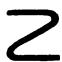
\includegraphics[keepaspectratio]{images/part001_149bf36b.jpg}}

于是，如果 E 是局部凸且可度量化的，且其拓扑不能由单个范数定义，那么 E 上不存在定义其拓扑且使对 \(d\) 而言的有界子集（GT, IX, § 2, No.~2）恰为 E 的有界子集的距离。更确切地说，对 E 上每个平移不变且定义 E 的拓扑的距离 \(d\) ，E 的有界子集对 \(d\) 而言是有界的（III, 第 38 页, 习题 3），但反之不真。

\begin{enumerate}
\def\labelenumi{\arabic{enumi})}
\setcounter{enumi}{1}
\item
  设 M 是 E 的一个向量子空间，赋有诱导拓扑。要使 M 的一个子集在 M 中有界，必须且只需它在 E 中有界。
\item
  设 N 是 E 中 0 的所有邻域之交，于是 \(\tilde{E} = E/N\) 是与 E 相伴的 Hausdorff 向量空间。那么 N 是有界的；如果 \(\pi: E \to \tilde{E}\) 是典范同态，那么 E 的子集 B 有界当且仅当 \(\pi(B)\) 有界。
\item
  设 E 是一个 Hausdorff 局部凸空间；那么对 E 中每个 \(x \neq 0\) ，存在一个连续半范数 p，使得 \(p(x) \neq 0\) ；这个半范数在由 x 生成的实半直线 \(R_{+}.x\) 上不是有界的。因此 E 的任何非零子空间都不是有界的。特别地，有界子集不含任何直线。
\end{enumerate}

定义 4. --- 设 E 是一个局部凸空间。E 上的有界结构 B 称为与 E 适配的，如果它是凸的，由 E 的有界子集组成，且 B 中每个集合的闭包属于 B。

命题 1. --- 设 E 是一个局部凸空间。E 的有界子集所成之集是一个适配有界结构。

我们需要确立下列性质：

\begin{enumerate}
\def\labelenumi{\alph{enumi})}
\item
  如果 \(\mathbf{B}\) 是 \(\mathbf{E}\) 的一个有界子集，那么 \(\mathbf{B}\) 的每个子集都有界。
\item
  两个有界子集的并是有界的。
\item
  与一个有界集位似的每个集合是有界的。
\item
  有界子集的闭均衡凸包（II, 第 13 页）是有界的。
\end{enumerate}

如果 p 是 E 上的一个连续半范数，那么 p 的球是凸的、均衡的、闭的，且与一个球位似的集合还是一个球。因此，如果 p 在 E 的两个子集 X 与 Y 上有界，那么它在 \(X \cup Y\) 的闭均衡凸包上、在与这些集合位似的集合上也都有界。这就确立了性质 b)、c) 与 d)，而 a) 是显然的。

定义 5. --- 设 E 是一个局部凸空间。E 的所有有界子集所成之集称为 E 的典范有界结构。

如果 B 是 E 的有界子集所成的一个集合，那么存在一个与 E 适配且包含 B 的最小有界结构 \(\tilde{B}\) 。\(\tilde{B}\) 中的集合就是那些含于某个集合的集合，该集合与 B 中集合的有限并的闭均衡凸包位似。

每个适配有界结构都含于典范有界结构之中。

命题 2. --- 在局部凸空间 E 中，每个预紧集是有界的。设 A 是 E 的一个预紧子集，V 是 0 的一个均衡凸邻域。存在 A 中点的一个有限序列 \((a_{i})_{1\leqslant i\leqslant n}\) ，使得

\[
\mathrm{A} \subset \bigcup_ {1 \leqslant i \leqslant n} (a _ {i} + \mathrm{V}).
\]

由于 \(B = \{a_{1}, ..., a_{n}\}\) 是有界的，存在一个标量 \(\lambda\) ，使得 \(0 < \lambda < 1\) 且 \(\lambda B \subset V\) ；我们有 \(\lambda A \subset \lambda B + \lambda V \subset V + V\) ，由此命题得证。

推论. --- 在局部凸空间中，一个 Cauchy 序列的点所成之集是有界的。

事实上，这个集合是预紧的（GT, II, § 4, No.~2）。

注 5. --- 一般说来，局部凸空间 E 的有界子集并不都是预紧的（例如，如果 E 是无限维赋范空间，其单位球不是紧的（I, 第 15 页, 定理 3））。然而，当 E 是弱空间（II, 第 42 页）时情形就是如此：因为这时与 E 相伴的 Hausdorff 拓扑向量空间同构于某个乘积 \(K^{I}\) 的子空间，而该乘积的有界子集都是预紧的（参见 III, 第 4 页, 推论 2）。

其他的例子见 IV, 第 18 页。

命题 3. --- 设 A 是局部凸空间 E 的一个子集。假设 A 有界；那么对 A 中点的每个序列 \((x_{n})\) 以及趋于 0 的标量的每个序列 \((\lambda_{n})\) ，序列 \((\lambda_{n}x_{n})\) 趋于 0。反之，如果存在非零标量的一个序列 \((\lambda_{n})\) ，使得对 A 中点的每个序列 \((x_{n})\) ，序列 \((\lambda_{n}x_{n})\) 有界，那么 A 有界。

假设 A 有界。如果 \((\lambda_{n})\) 是趋于 0 的标量序列，且 V 是 0 的一个邻域，那么当 n 充分大时有 \(\lambda_{n}A \subset V\) ，由此第一个断言得证。

反之，如果 A 不是有界的，且 \((\lambda_{n})\) 是一个标量 \(\neq 0\) 的序列，那么存在一个连续半范数 p 与 A 中点的一个序列 \((x_{n})\) ，使得 \(p(x_{n}) \geqslant \frac{n}{|\lambda_{n}|}\) 。于是有 \(p(\lambda_{n}x_{n}) \geqslant n\) ，从而序列 \((\lambda_{n}x_{n})\) 不是有界的。

推论. --- E 的子集 A 有界，当且仅当 A 的每个可数子集有界。

\subsection{在连续映射下的像}

命题 4. --- 设 E 与 F 是两个局部凸空间，\(f:E \rightarrow F\) 是一个连续映射。假设 \(f(0) = 0\) ，且存在一个实数 \(m \geqslant 0\) ，使得 \(f(\lambda x) = \lambda^{m}f(x)\) 对每个 \(\lambda > 0\) 成立。那么，如果 A 是 E 的一个有界子集，则 \(f(A)\) 在 F 中有界。

事实上，如果 V 是 F 中 0 的一个邻域，那么 \(f^{-1}(V)\) 是 E 中 0 的一个邻域。如果 A 在 E 中有界，则存在 \(\lambda > 0\) ，使得 \(A \subset \lambda f^{-1}(V)\) ，这蕴含 \(f(A) \subset \lambda^{m}V\) 。

推论 1. --- 设 E 与 F 是两个局部凸空间，\(u:E\to F\) 是一个连续线性映射。如果 A 是 E 的一个有界子集，那么 \(u(A)\) 在 F 中有界。

推论 2. --- 设 \(\mathrm{E} = \prod_{i\in \mathrm{I}}\mathrm{E}_i\) 是一个局部凸空间族的乘积。

那么 E 的一个子集有界，当且仅当它的所有投影都有界。更一般地：

推论 3. --- 设 E 是一个向量空间，\((\mathrm{F}_{i})_{i\in\mathrm{I}}\) 是一个局部凸空间族，\(f_{i}\) 是从 E 到 \(F_{i}\) 中的一个线性映射（对每个 \(i\in I\) ）。假设给 E 装备使所有 \(f_{i}\) 都连续的最粗（局部凸）拓扑（II, 第 26 页）。那么，要使 E 的子集 A 有界，必须且只需 \(f_{i}(A)\) 在 \(F_{i}\) 中有界（对所有 \(i\in I\) ）。

事实上，如果 A 有界，那么诸 \(f_{i}(\mathbf{A})\) 也有界（推论 1）。反之，如果诸 \(f_{i}(\mathbf{A})\) 有界，且 p 是 E 上的一个连续半范数，那么存在 I 的一个有限子集 J 与一个族 \((q_{j})_{j\in \mathbb{J}}\) ，其中 \(q_{j}\) 是 \(\mathbf{F}_j\) 上的一个连续半范数，使得 \(p\leqslant \sup_{j\in \mathbb{J}}(q_j\circ f_j)\) ，因而 \(p\) 在 \(\mathbf{A}\) 上有界。

推论 4. --- 设 \(\mathbf{E}_i\) ( \(1 \leqslant i \leqslant n\) ) 与 \(\mathbf{F}\) 是局部凸空间，\(f\) 是从 \(\prod_{i=1}^{n} \mathbf{E}_i\) 到 \(\mathbf{F}\) 中的一个连续多重线性映射。如果 \(\mathbf{B}_i\) 是 \(\mathbf{E}_i\) 的一个有界子集（对 \(1 \leqslant i \leqslant n\) ），那么 \(f\left(\prod_{i=1}^{n} \mathbf{B}_i\right)\) 在 \(\mathbf{F}\) 中有界。

推论 5. --- 设 E 与 F 是两个局部凸空间，\(u:E\to F\) 是一个连续多项式映射。如果 A 是 E 的一个有界子集，那么 \(u(A)\) 有界。

\subsection{某些归纳极限中的有界子集}

命题 5. --- 设 \((\mathrm{E}_{i})_{i\in\mathbf{I}}\) 是一个 Hausdorff 局部凸空间族，E 是这个族的拓扑直和（II, 第 29 页）。要使 E 的子集 B 有界，必须且只需存在 I 的一个有限子集 J，使得 \(\operatorname{pr}_{i}(\mathbf{B})\) 在 \(E_{i}\) 中有界（对 \(i\in J\) ），且 \(\operatorname{pr}_{i}(\mathbf{B})\subset\{0\}\) 对所有 \(i\notin J\) 成立。

设 J 是 I 的一个有限子集。由于 E 的拓扑在 \(\prod_{j\in J}E_{j}\) 上诱导乘积拓扑（II, 第 30 页, 命题 7 与第 31 页, 命题 8），由 III, 第 4 页, 推论 2 即知该条件是充分的。

反之，设 B 是 E 的一个有界子集。那么 \(\mathrm{pr}_{i}(\mathbf{B})\) 对所有 i 有界（III, 第 4 页, 推论 1）。因此只需证明存在 I 的一个有限子集 J，使得 \(\mathrm{pr}_{i}(\mathbf{B}) \subset \{0\}\) 对所有 \(i \notin J\) 成立。若不然，则存在 I 的互异元素的一个无穷序列 \((i_{n})\) 与 B 的元素的一个无穷序列 \((x_{n})\) ，使得 \(\mathrm{pr}_{i_{n}}(x_{n}) \neq 0\) 。由于 \(E_{i_{n}}\) 是 Hausdorff 的，存在一个连续半范数 \(p_{n}\) （\(E_{i_{n}}\) 上的），使得 \(p_{n}(\mathrm{pr}_{i_{n}}(x_{n})) \geqslant n\) 。于是 \(p = \sum_{n \geqslant 1} p_{n} \circ \mathrm{pr}_{i_{n}}\) 是 E 上的一个连续半范数，且 p 在 B 上不是有界的，这就得到矛盾。

命题 6. --- 设 E 是一个局部凸空间，它是 E 的闭向量子空间的一个递增序列 \((E_{n})\) 的严格归纳极限（II, 第 33 页）。E 的子集 B 有界，当且仅当它含于某个子空间 \(E_{n}\) 之中，且在这个子空间中有界。

该条件是充分的，因为 E 的拓扑在 \(E_{n}\) 上诱导的拓扑正是 \(E_{n}\) 上给定的拓扑（II, 第 32 页, 命题 9）。要看出该条件是必要的，只需（III, 第 4 页, 命题 3）证明：如果 E 的点的一个序列 \((x_{m})\) 不含于任何子空间 \(E_{n}\) 之中，那么它不能趋于 0。通过抽取序列 \((x_{m})\) 的一个子序列，我们可以假设存在一个严格递增的整数序列 \((n_{k})\) ，使得对每个指标 k，有 \(x_{k} \notin E_{n_{k}}\) 且 \(x_{k} \in E_{n_{k+1}}\) 。那么存在（II, 第 33 页, 引理 2）凸集的一个递增序列 \((V_{k})\) ，使得 \(V_{k}\) 是 \(E_{n_{k}}\) 中 0 的一个邻域，\(V_{k+1} \cap E_{n_{k}} = V_{k}\) ，且对每个指标 k 有 \(x_{k} \notin V_{k+1}\) 。于是诸 \(V_{k}\) 的并 V 是 E 中 0 的一个邻域，且对所有 k 有 \(x_{k} \notin V\) 。这就证明序列 \((x_{k})\) 不趋于 0。

对空间 \(\mathbf{E}\) （它是 \(\mathrm{E}\) 的闭子空间的一个不可数有向集的归纳极限），命题 6 的结论未必成立（参见 III, 第 38 页, 习题 7）。

命题 7. --- 设 \((\mathrm{E}_{n})_{n\geq0}\) 是一个 Hausdorff 局部凸空间序列，且对每个 n，设 \(u_{n}:E_{n}\to E_{n+1}\) 是一个单射的紧线性映射（即：存在 \(E_{n}\) 中 0 的一个邻域，它在 \(u_{n}\) 下的像是相对紧的；这蕴含 \(u_{n}\) 连续）。设 E 是系统 \((\mathrm{E}_{n},u_{n})\) 的归纳极限（II, 第 29 页），且设 \(v_{n}\) 是从 \(E_{n}\) 到 E 中的典范映射。那么局部凸空间 E 是 Hausdorff 的。此外，对 E 的每个子集 A，下列条件等价：

\begin{enumerate}
\def\labelenumi{(\roman{enumi})}
\item
  A 是有界的；
\item
  存在一个整数 \(n\) ，使得 \(\mathbf{A}\) 是在 \(v_{n}\) 之下 \(\mathrm{E}_n\) 的一个有界子集的像；
\item
  A 是相对紧的。
\end{enumerate}

我们把 \(\mathbf{E}_n\) 与 \(\mathbf{E}\) 的一个向量子空间视为同一（它赋有一个比诱导拓扑更细的拓扑）。

引理 1. --- 在命题 7 的假设下，E 的拓扑是使所有映射 \(v_{n} : \mathrm{E}_{n} \to \mathrm{E}\) 都连续的最细拓扑。

我们需要证明：如果 U 是 E 的一个子集，使得 \(U \cap E_{n}\) 对每个 n 在 \(E_{n}\) 中是开的，那么 U 在 E 中是开的；换言之，我们必须证明，对每个 \(x \in U\) ，存在一个均衡凸集 V，使得 \(x + V \subset U\) ，且 \(V \cap E_{n}\) 对所有充分大的 n 是 \(E_{n}\) 中 0 的一个邻域（II, 第 27 页, 命题 5）。对每个 n，设 \(W_{n}\) 是 \(E_{n}\) 中 0 的一个均衡凸邻域，使得 \(H_{n}\) （即 \(W_{n}\) 在 \(E_{n+1}\) 中的闭包）是紧的。设 \(x \in U\) ，并设 \(n_{0}\) 是一个使得 \(x \in E_{n_{0}}\) 的整数。我们将用归纳法构造标量的一个序列 \((\varepsilon_{n})_{n \geqslant 0}\) （\textgreater0），使得 \(x + \sum_{n_{0} \leqslant i \leqslant n} \varepsilon_{i}H_{i}\) 对 \(n \geqslant n_{0}\) 含于 U 中。假设诸 \(\varepsilon_{i}\) （对 i \textless{} n）已经构造出来。如果 \(n = n_{0}\) ，令 \(V_{n-1} = \{0\}\) ；否则令

\[
\mathrm{V} _ {n - 1} = \sum_ {n _ {0} \leqslant i \leqslant n - 1} \varepsilon_ {i} \mathrm{H} _ {i}.
\]

那么 \(V_{n-1}\) 在 \(E_{n}\) 中是紧的，从而在 \(E_{n+1}\) 中更是紧的。由于 \(U \cap E_{n+1}\) 在 \(E_{n+1}\) 中是开的，存在一个标量 \(\varepsilon_{n} > 0\) ，使得 \(x + V_{n} = x + V_{n-1} + \varepsilon_{n}H_{n}\) 含于 U 中（GT, II, §4, No.~3, cor.）。令 \(V = \bigcup_{n \geqslant n_{0}} V_{n}\) 。那么 V 是凸的且均衡的；对 \(n \geqslant n_{0}\) ，我们有 \(V \cap E_{n} \supset \varepsilon_{n}H_{n} \cap E_{n} \supset \varepsilon_{n}W_{n}\) ，因而 \(V \cap E_{n}\) 是 \(E_{n}\) 中 0 的一个邻域。这样就完成了引理的证明。

集合 \(\mathrm{U} = \mathrm{E} - \{0\}\) 具有这样的性质：集合 \(\mathrm{U} \cap \mathrm{E}_n = \mathrm{E}_n - \{0\}\) 在 \(\mathrm{E}_n\) 中是开的（对每个 \(n\) ），因而 \(\mathrm{U}\) 在 \(\mathrm{E}\) 中是开的，这就证明 \(\mathrm{E}\) 是 Hausdorff 的（GT, III, § 1, No.~3, prop. 2）。显然性质 (ii) 蕴含 (iii)，且 (iii) 蕴含 (i)。最后我们证明 (i) 蕴含 (ii)。为此只需证明：如果 \(\mathrm{A}\) （\(\mathrm{E}\) 的一个子集）不被诸集合 \(\sum_{0 \leqslant i \leqslant n} \mathrm{H}_i\) 中任何一个吸收，那么 \(\mathrm{A}\) 不是有界的。但这时存在一个序列 \((x_n)_{n \geqslant 1}\) （由 \(\mathrm{A}\) 的点组成），使得对每个 \(n\) ，有 \(x_n \notin n^2 \sum_{0 \leqslant i \leqslant n} \mathrm{H}_i\) 。

那么诸 \(x_{n}/n\) 所成之集依引理 1 是闭的，因为它与 \(E_{m}\) 的交对每个整数 m 都是离散的。于是诸 \(x_{n}/n\) 所成之集的补集是 0 的一个开邻域，它不吸收序列 \((x_{n})\) ，因而 A 不是有界的。

注. --- 1) 用上面的记号，设 \(F_{n}\) 是由 \(H_{n}\) 生成的向量空间，赋以等于 \(H_{n}\) 的度规的范数。我们将看到（III, 第 8 页, cor.），\(F_{n}\) 是一个 Banach 空间。从 \(F_{n}\) 到 \(E_{n+1}\) 中的单射是紧的，因而单射 \(w_{n}\) （从 \(F_{n}\) 到 \(F_{n+1}\) 中的单射）更是紧的。此外，E 是 Banach 空间的归纳系统 ( \(F_{n}, w_{n}\) ) 的归纳极限。事实上，E 中 0 的一个均衡凸邻域 V 满足：\(V \cap E_{n}\) 吸收 \(H_{n-1}\) （对所有 \(n \geqslant 1\) ）；反之，如果 E 中的一个均衡凸集 W 满足 \(W \cap E_{n}\) 吸收 \(H_{n-1}\) ，那么 \(W \cap E_{n-1}\) 含有一个与 \(W_{n-1}\) 位似的集合（对所有 \(n \geqslant 1\) ），从而 W 是 E 中 0 的一个邻域。

\begin{enumerate}
\def\labelenumi{\arabic{enumi})}
\setcounter{enumi}{1}
\tightlist
\item
  设 F 是一个局部凸空间，k 是一个整数 \(\geqslant0\) ，\(f:E^{k}\rightarrow F\) 是一个多重线性映射。要使 f 连续，必须且只需 f 在 \(E_{n}^{k}\) 上的限制对每个 n 连续。我们立即验证：\(E^{k}\) 对线性映射族 \(v_{n}\times\cdots\times v_{n}:E_{n}\times\cdots\times E_{n}\to E\times\cdots\times E\) 具有终局部凸拓扑（II, 第 28 页, cor. 2 与第 30 页, 命题 7），且 \(u_{n}\times\cdots\times u_{n}\) 是从 \((\mathrm{E}_{n})^{k}\) 到 \((\mathrm{E}_{n+1})^{k}\) 中的一个紧单射线性映射。现在只需应用引理 1。
\end{enumerate}
